\documentclass{beamer}

\usepackage[english]{babel}
\usepackage[utf8x]{inputenc}
\usepackage{amsmath,amsfonts,amssymb}

\usepackage{mathtools}





\usepackage{subcaption}

\usepackage[absolute,overlay]{textpos}





\newcommand{\todo}[1]{\textcolor{red}{TODO: #1}}
\newcommand{\var}{\operatorname{Var}}


\addtobeamertemplate{navigation symbols}{}{%
    \usebeamerfont{footline}%
    \usebeamercolor[fg]{footline}%
    \hspace{1em}%
    \insertframenumber/\inserttotalframenumber
}

\setbeamertemplate{bibliography item}[text]
\bibliographystyle{unsrt}


\usetheme{Luebeck}
\usecolortheme{orchid}




\title[Current state of master thesis]{Modeling, numerical simulation \\ and parameter estimation in \\ heat flux differential scanning calorimetry}
\subtitle{Current state of master thesis}

\author{Jan Lammel}

\begin{document}
	
\frame{\titlepage}

\frame{
	\frametitle{Table of contents}
	\tableofcontents[hideallsubsections]
	
}

\section{Introduction}
\frame{
\frametitle{Introduction}

	\begin{textblock}{7}(1,5)
		\includegraphics[width=1.0\textwidth]{/home/argo/masterarbeit/thesis/images/handwaermer[wiki].jpg} \\
		\qquad \quad Source: Wikipedia
	\end{textblock}
	
	\begin{textblock}{8}(8,5)
	\begin{itemize}
		\item We examine so called phase change materials (PCM).
		\item Important property is the heat capacity $c_p$: When does it melt and how much energy fits into?
	\end{itemize}
	\end{textblock}

	\begin{textblock}{14}(1,12.5)

	\textbf{Goal:} Simulation of measuring process to obtain specific heat capacity $c_p$ of phase change material (PCM) by parameter estimation.

	\end{textblock}
	

}

\section{Physical background}
\subsection{Important physical quantities}
\frame{
	\frametitle{Important physical quantities}
	
	\begin{textblock}{15}(0.3,4.2)
		\begin{itemize}
			\item Heat $Q$, \qquad $[Q] = J$ \\
			Amount of energy transferred because of temperature difference. \\ \vspace{0.2cm}
			
			\item heat flux density $\Phi_q$, \qquad$[\Phi_q] = \frac{W}{m^2}$ \\
			Rate of energy transferred per unit area. \\
			$\rightarrow$ heat flux: $\varPhi_q$
			\vspace{0.2cm} 
			
			\item heat conductivity $\lambda$, \qquad $[\lambda] = \frac{W}{m \cdot K}$ \\
			Material property: Amount of energy being transported on a distance of $1m$ (unit area) at a temperature difference of $1K$ in $1s$. \vspace{0.2cm}
			
			\item specific heat capacity $c_p$, \qquad $[c_p] = \frac{J}{kg \cdot K}$ \\
			Material property: Amount of energy needed to raise the temperature of $1kg$ by $1K$.
			
		\end{itemize}
	\end{textblock}
	
}


\subsection{Heat flux differential scanning calorimetry (DSC)}
\frame{
	\frametitle{Heat flux differential scanning calorimetry (DSC)}
	
	\begin{textblock}{15}(0.4,4)
		\centering
		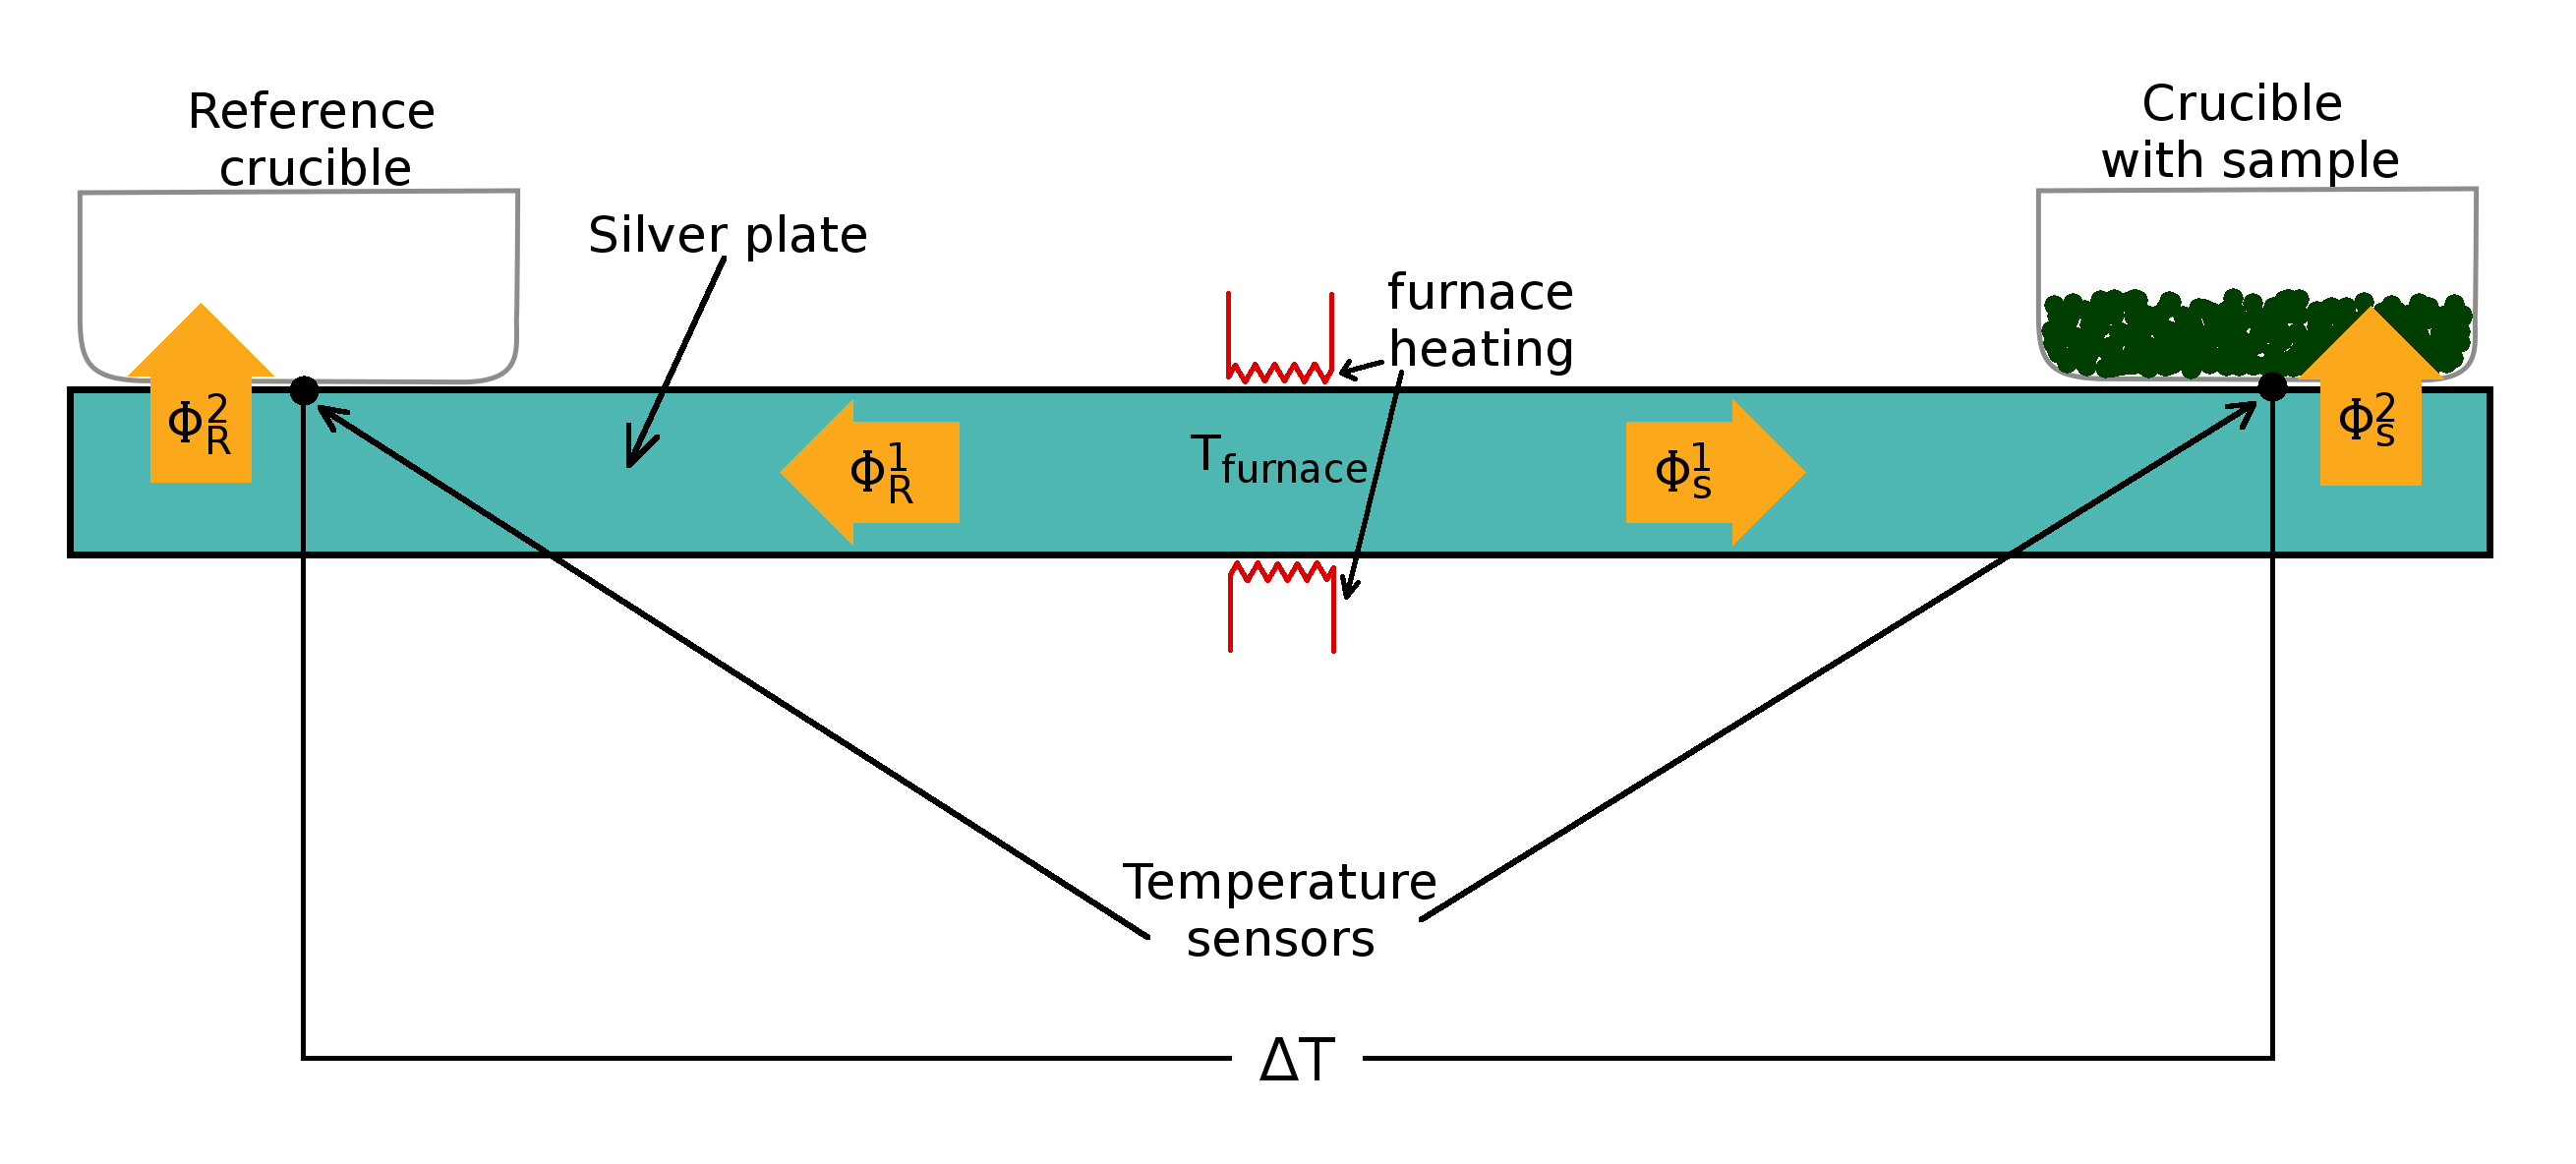
\includegraphics[width=0.7\textwidth]{/home/argo/masterarbeit/thesis/images/dsc_funktionsprinzip.png}
		
		\begin{itemize}
			\item Empty reference crucible and crucible with PCM are heated equally.
			\item Due to thermal properties differences (mainly $c_p$) of reference and PCM a temperature difference $\Delta T$ is induced.
			\item Sensitivity calibration with materials of known thermal properties provides mapping $\Delta T \rightarrow \varPhi_q$.
		\end{itemize}
		
	\end{textblock}
	
}


\subsection{Smearing problem}
\frame{
	\frametitle{Smearing problem}	
	
	\begin{textblock}{10}(0.5,5)
		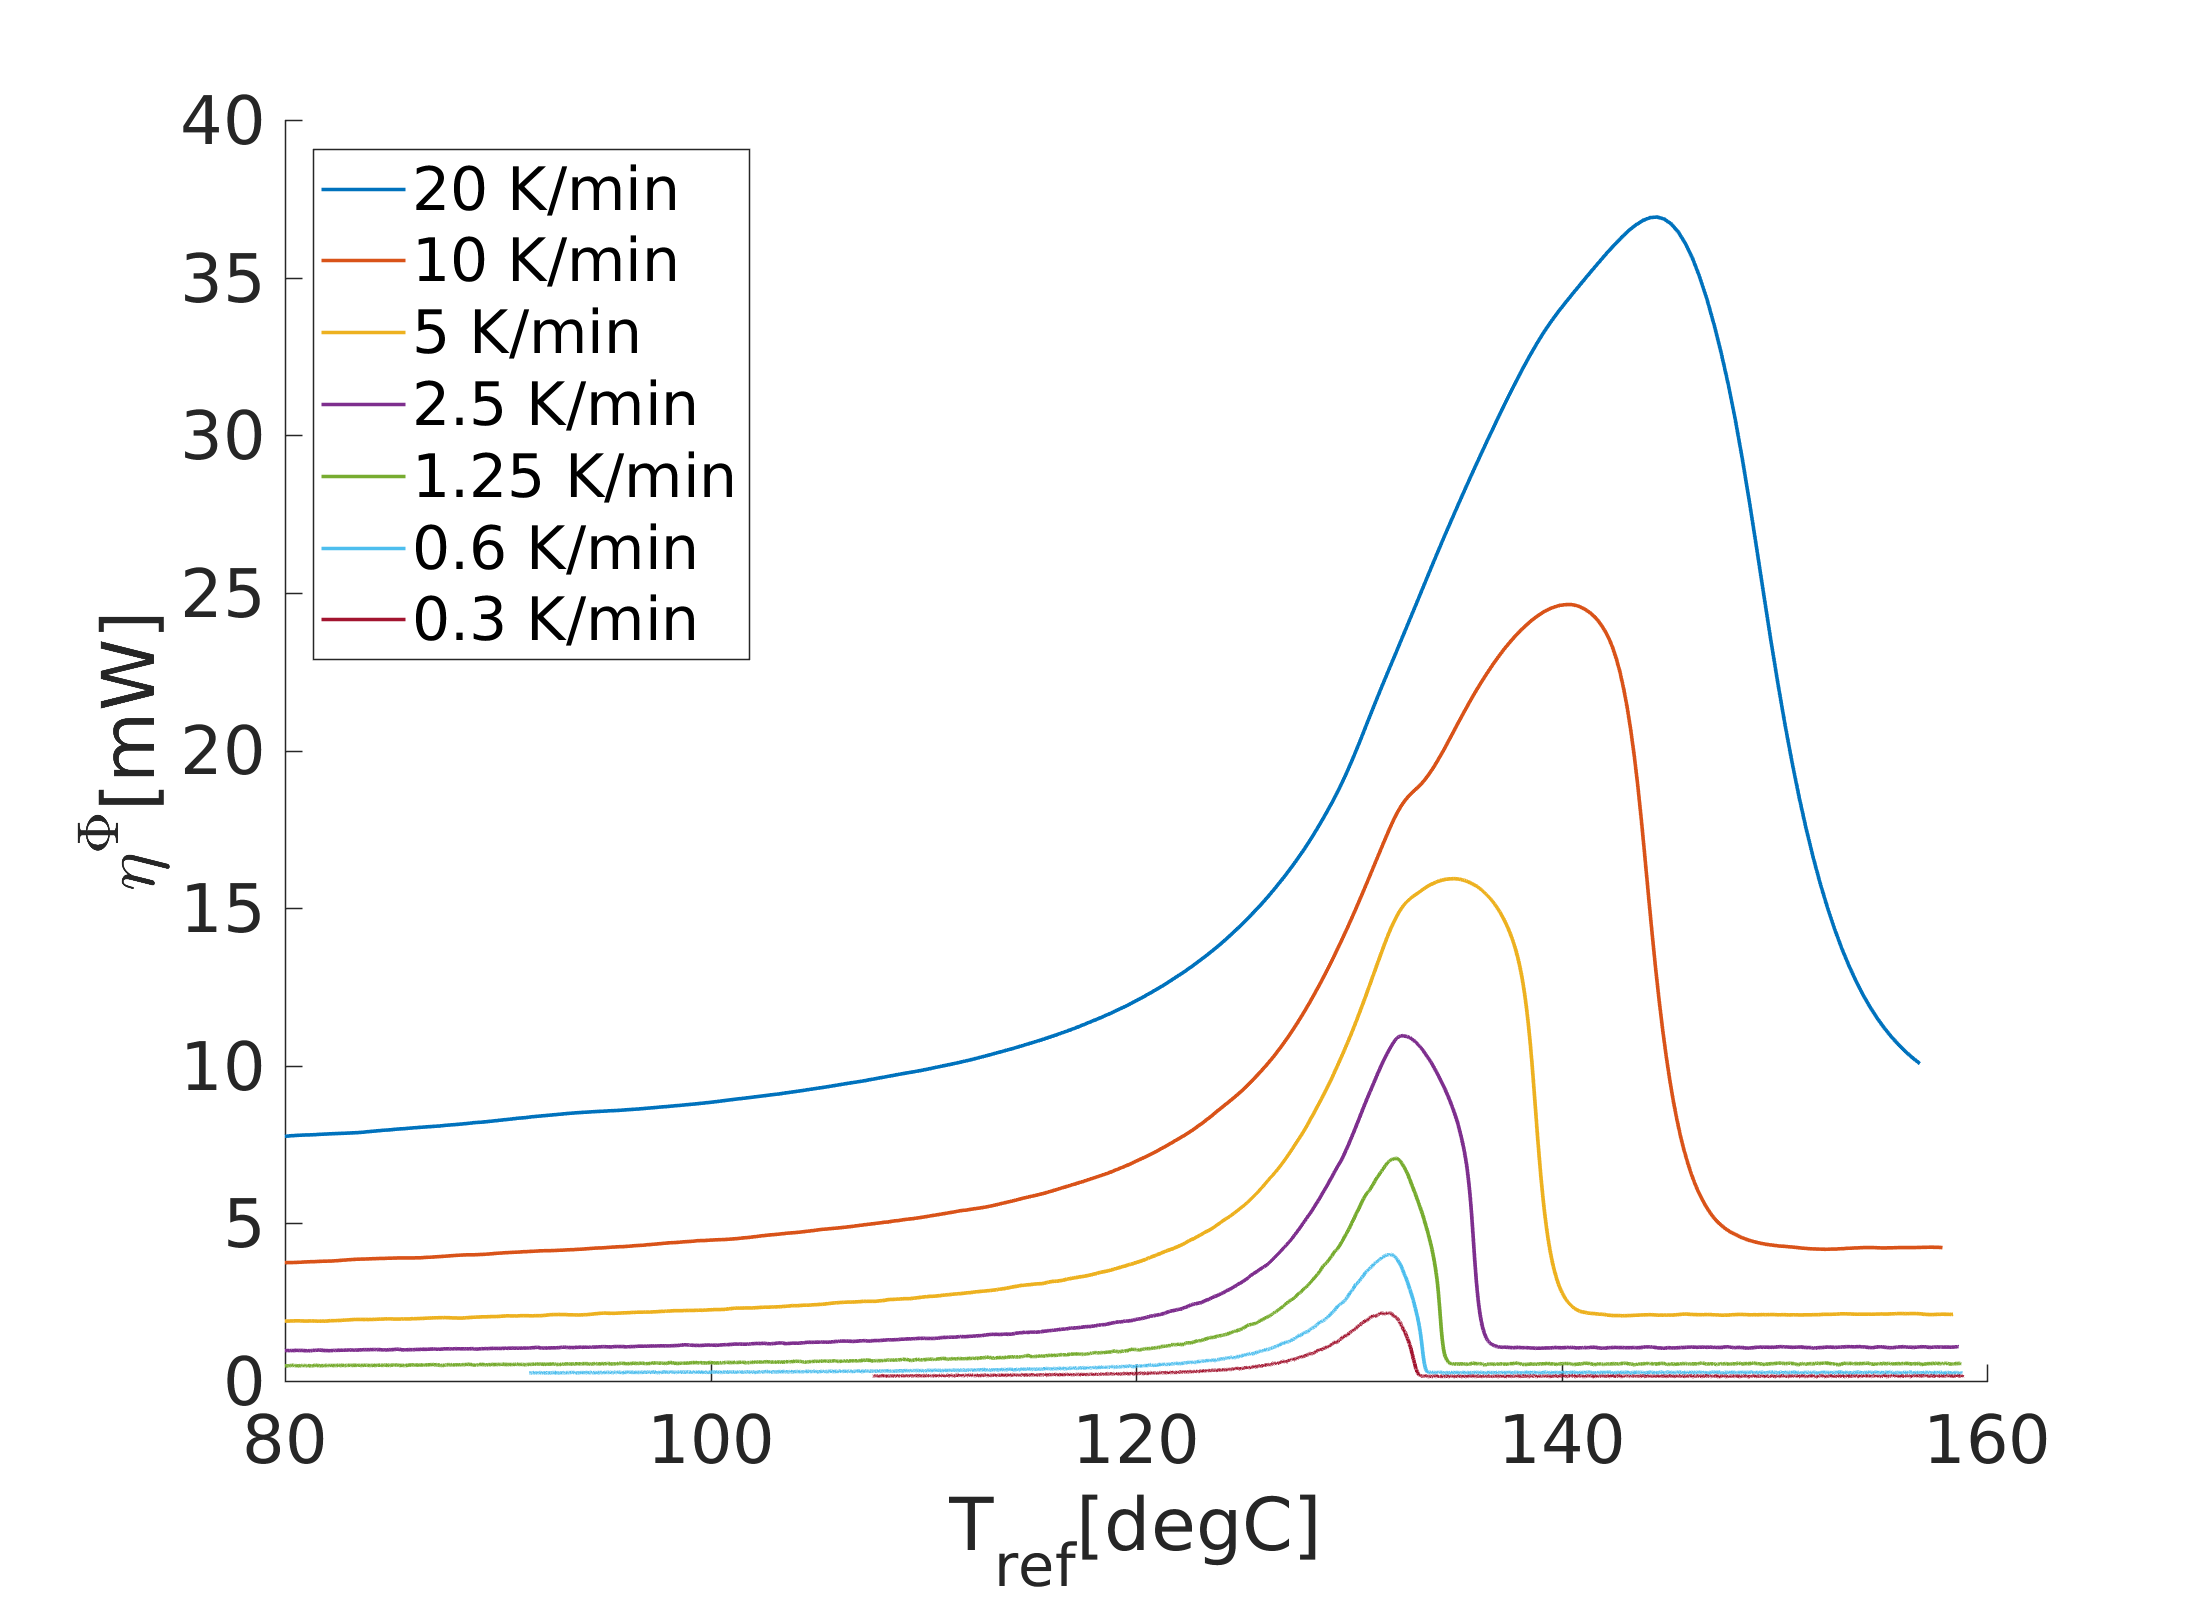
\includegraphics[width=0.7\textwidth]{/home/argo/masterarbeit/thesis/images/heat_flux_measurement.png}
	\end{textblock}
	
	\begin{textblock}{4}(7.5,8)
		$\stackrel{(1)}{\longrightarrow}$
	\end{textblock}
	
	\begin{textblock}{10}(8.7,5)
		\includegraphics[width=0.7\textwidth]{/home/argo/masterarbeit/thesis/images/c_p_DIN_formula.png}
	\end{textblock}
	
	\begin{textblock}{14}(1,12)
		\begin{equation}
			\text{DIN 11357: } \quad c_p^{DIN}(T) = c_p^{R}(T) \cdot \frac{m^R}{m^S} \cdot \frac{\Phi^S(T) - \Phi^0(T)}{\Phi^R(T) - \Phi^0(T)}
		\end{equation}
	\end{textblock}
	
}


\section{Mathematical model \& parameter estimation}
\subsection{Mathematical model}
\frame{
	\frametitle{Mathematical model}
	
	\begin{textblock}{14}(1, 3.9)
		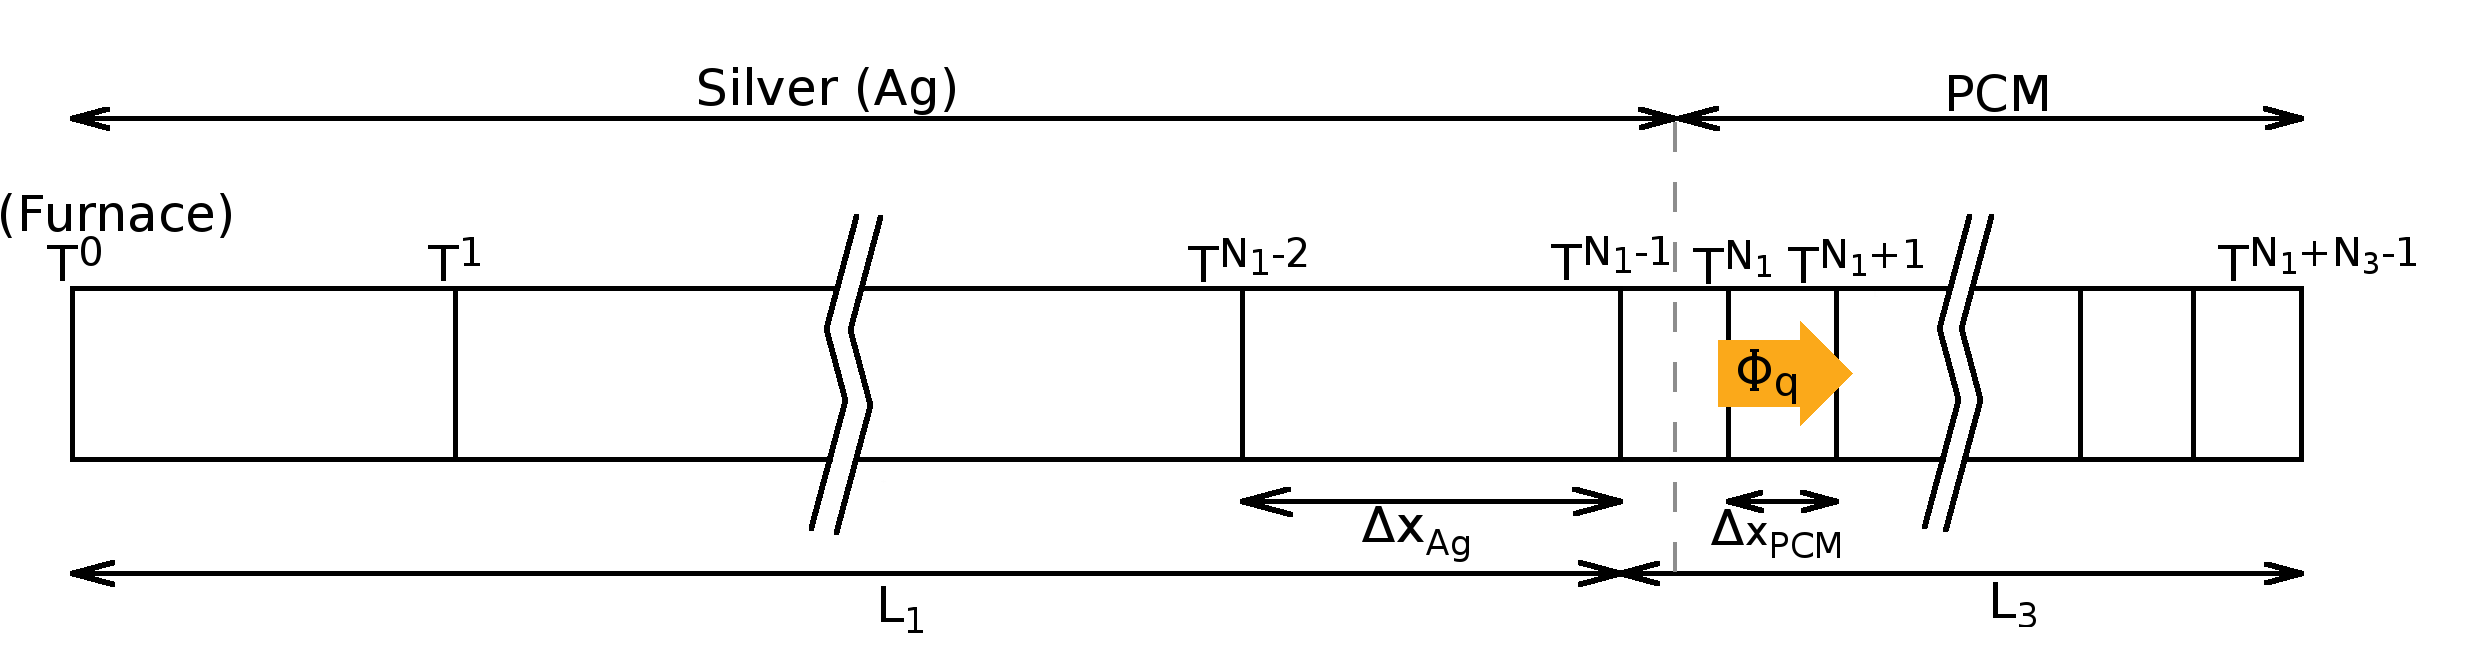
\includegraphics[width=1.\textwidth]{/home/argo/masterarbeit/thesis/images/discretization_grid_heat_flux.png}
	\end{textblock}
	
	
	\begin{textblock}{14}(0.4, 8.8)
	
		\begin{itemize}
			\item Heat equation: \quad $\rho c_p(T(x,t)) \frac{\partial T}{\partial t}(x,t) = \nabla \cdot \left[ \lambda \cdot \nabla T(x,t) \right]$
			\item $\rho$, $\lambda$ constant
			\item Boundary conditions: 
				\begin{itemize}
				\item $T^0 = T_0 + \beta \cdot t$ \\
				\item No flux outside PCM
				\end{itemize}
			\item Reference and PCM side are independent
			\item Spatial discretization by method of lines
			
		\end{itemize}
	\end{textblock}
	
	\begin{textblock}{7}(8,10.35)
		\begin{itemize}
			\item Initial condition: 
			\begin{itemize}
				\item $T^i(t_0)=T_0 \ \forall \ i$
			\end{itemize}
		\end{itemize}
	\end{textblock}

	
}


\frame{

	\begin{textblock}{12}(1.8, 2.5)
		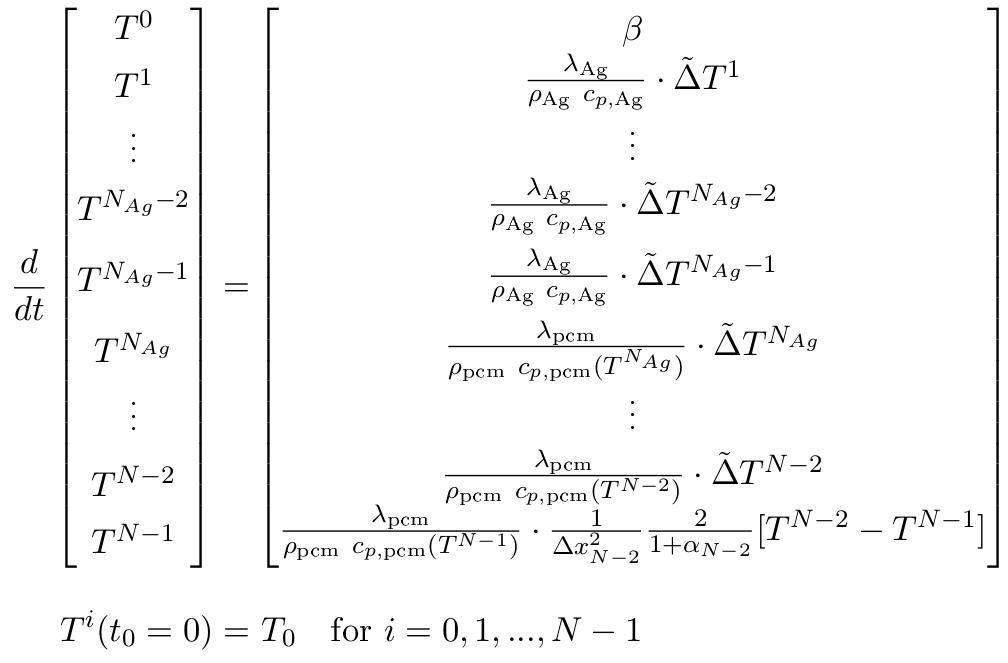
\includegraphics[width=1.0\textwidth]{/home/argo/masterarbeit/vortrag/images/model_IVP.png}
	\end{textblock}
	
	\begin{textblock}{12}(1,13.5)
		 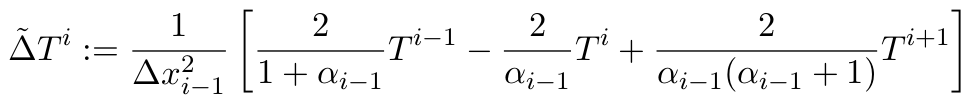
\includegraphics[width=1.0\textwidth]{/home/argo/masterarbeit/vortrag/images/discretized_2nd_derivative_in_IVP.png}
	\end{textblock}
}


\frame{
	\frametitle{Heat flux computation}	
	
	\begin{textblock}{14}(1,4.5)
		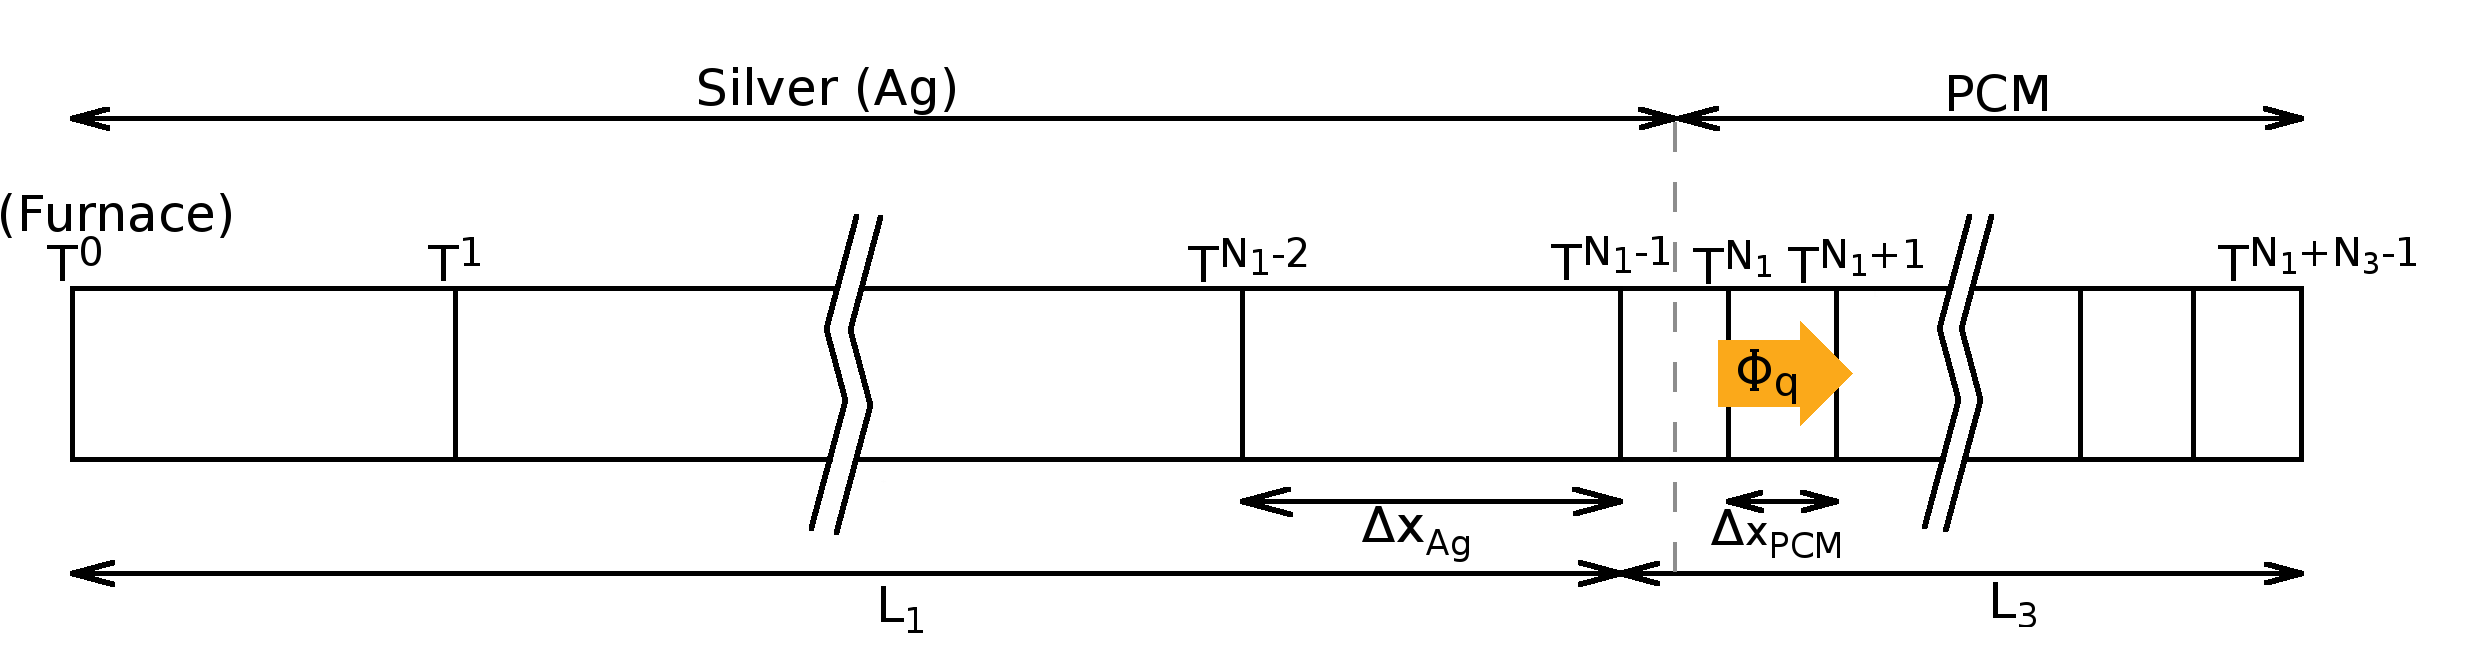
\includegraphics[width=1.\textwidth]{/home/argo/masterarbeit/thesis/images/discretization_grid_heat_flux.png}
	\end{textblock}
	
	\begin{textblock}{14}(1, 10)
		\begin{itemize}
			\item Heat flux into PCM: \\ \vspace{0.15cm}
			$\varPhi_{q}^{pcm,in} \approx - \bar{\lambda} \frac{T^{N_{Ag}} - T^{N_{Ag}-1}}{\Delta x_{N_{Ag}-1}} \cdot A_{pcm}
			\approx - \lambda_{pcm} \frac{T^{N_{Ag}+1} - T^{N_{Ag}}}{\Delta x_{N_{Ag}}} \cdot A_{pcm}$ \\ \vspace{0.15cm}
			where for the cross section $A_{pcm}$ we used $m_{N_{Ag}} = \rho_{pcm} \cdot A_{pcm} \cdot \Delta x_{N_{Ag}}$
		\end{itemize}
	\end{textblock}
	
}



%\frame{
%	\frametitle{Grid generation}
%
%	\begin{textblock}{10}(0.5,5)
%		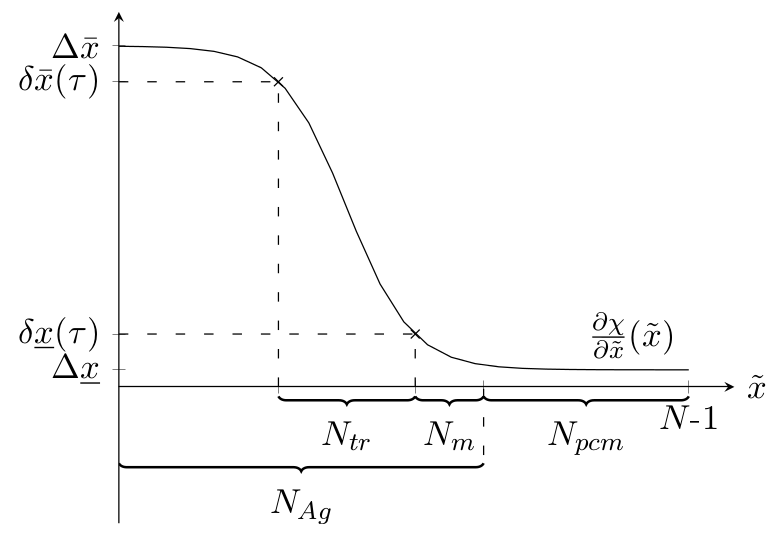
\includegraphics[width=1.0\textwidth]{/home/argo/masterarbeit/vortrag/images/grid_generation.png}
%	\end{textblock}
%	
%}




\subsection{Parametrization $c_p$}
\frame{
	\frametitle{Linear combination of Gaussians}
	
	\begin{textblock}{14}(1,4.5)
		\begin{equation*}
			c_p(T) = \sum_{i=1}^{5} A_i \exp\left(- \frac{(T - T_{\text{offset}_i})^2}{\var_i}\right) + m \cdot T + b
		\end{equation*}
	\end{textblock}
	
	\begin{textblock}{8}(1,7)
		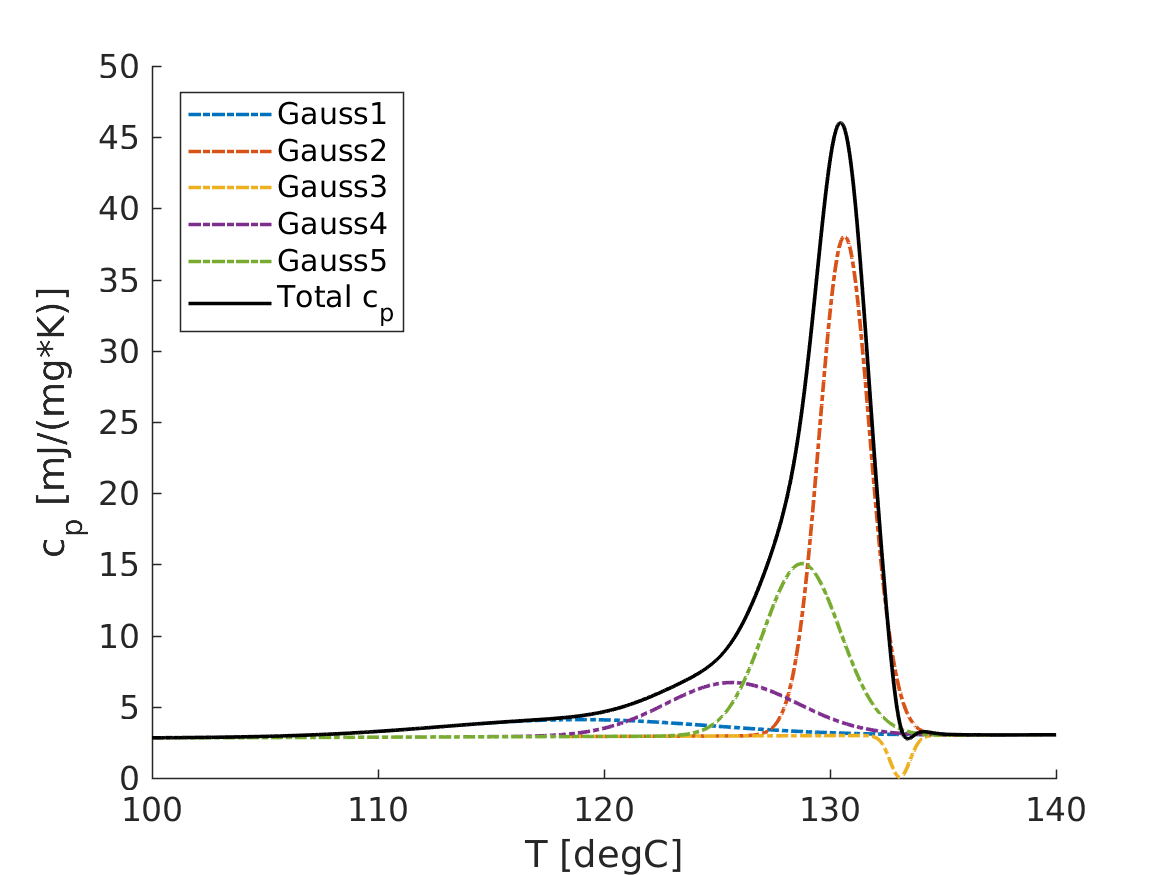
\includegraphics[width=1.0\textwidth]{/home/argo/masterarbeit/thesis/images/c_p_example.png}
	\end{textblock}
	
	\begin{textblock}{7}(8.5,7)
		\begin{itemize}
			\item Parameter: \\
			$A_i$, $T_{offset_i}$ and $\var_i$ for Gaussian i \\
			$m$ and $b$ for linear baseline
			\item In total $17$ parameter 
		\end{itemize}
	\end{textblock}
	
}


\frame{
	\frametitle{Fraser-Suzuki peak}
	
	\begin{textblock}{15.5}(0.2,4.3)
		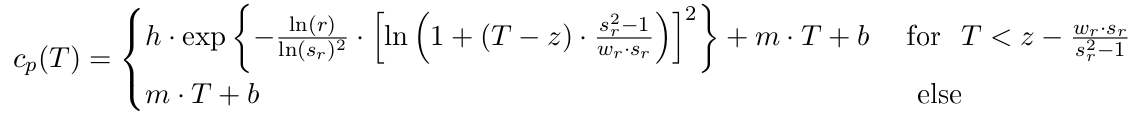
\includegraphics[width=1.0\textwidth]{/home/argo/masterarbeit/vortrag/images/fs_formula.png}
	\end{textblock}
	
	\begin{textblock}{8}(0.5,7)
		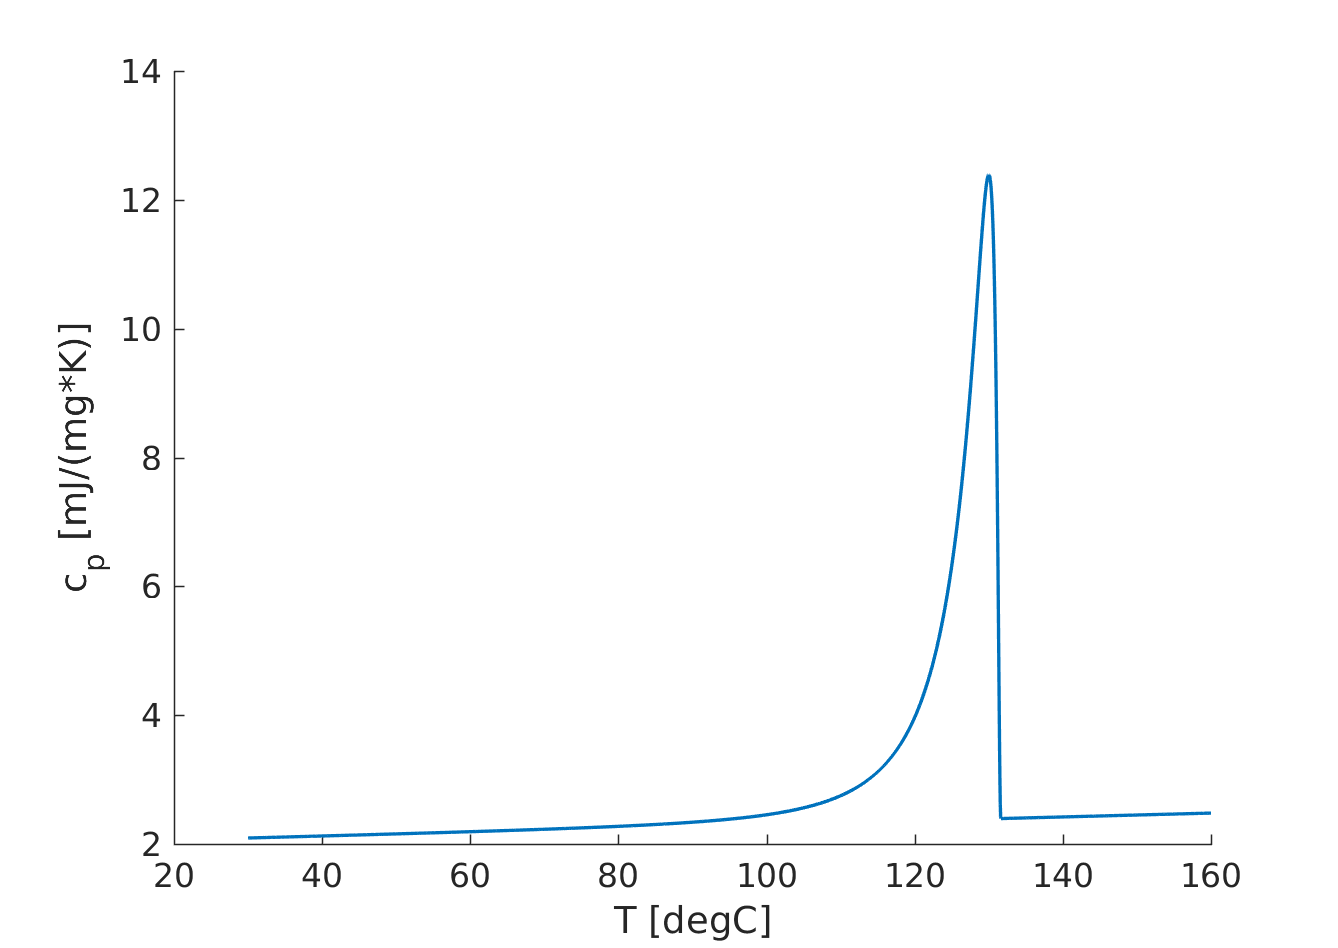
\includegraphics[width=1.0\textwidth]{/home/argo/masterarbeit/thesis/images/fraser_suzuki_example.png}
	\end{textblock}
	
	\begin{textblock}{7}(8.5,8)
		\begin{itemize}
			\item Parameter: \\
			$h$, $w_r$, $s_r$, $z$ for \\
			Fraser-Suzuki peak
			\item fixed $r=2$ for identifiability
			$m$ and $b$ for linear baseline
			\item In total $6$ parameter 
		\end{itemize}
	\end{textblock}
	
}




\subsection{Optimization problem}


\frame{
	\frametitle{Measurement time points computation}
	
	\begin{textblock}{8.5}(0.35,5)
		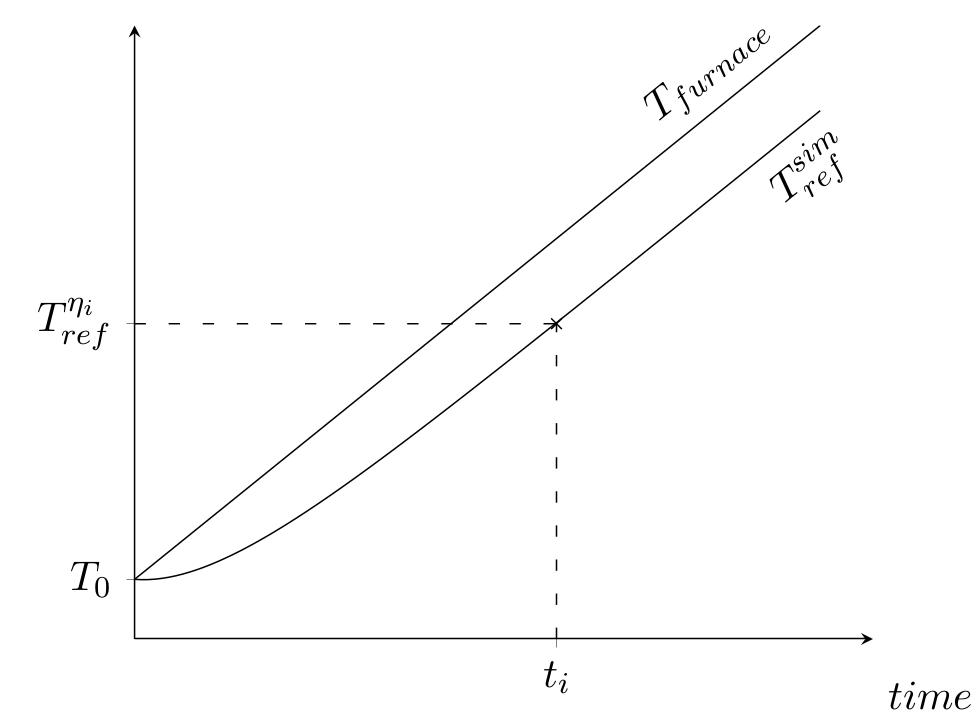
\includegraphics[width=1.\textwidth]{/home/argo/masterarbeit/vortrag/images/measurement_time_computation2.png}
	\end{textblock}
	
	\begin{textblock}{6.8}(8.5,5.)
	\begin{itemize}
		\item Reference side $T_{ref}^{sim}(t)$ is solved analytically. \\[2ex]
		\item Given heat flux measurement values $\varPhi_q^{\eta_i} = \varPhi_q^{\eta_i}(T_{ref}^{\eta_i})$. \\[1ex]
		$\rightarrow$ For fixed $T_0$ we can compute points in time $t_i$ where measurements were done using Newton's method.
	\end{itemize}
	\end{textblock}

	
}



\frame{
	\frametitle{Optimization problem}	


	\begin{textblock}{10}(0.5,4.)
	\begin{align*}
		\min_{p_{c_p}} \ & \sum_{i=1}^{n_{mp}} \left|\left|  \varPhi_{q}^{pcm,in}(T(t_i;T_0,p_{c_p})) - \varPhi_q^{\eta_i} \right|\right|_2^2 \\
		s.t. \ & \quad \  \dot{T} = f(T,t;p_{c_p}) \\
		       & T(0) = T_0
	\end{align*}
	\end{textblock}
	
	\begin{textblock}{7}(12,6.5)
		separately for all \\
		 heat rates $\beta$
	\end{textblock}
	
	\begin{textblock}{16}(0.3,9.4)
	\begin{itemize}
		\item $\varPhi_q^{\eta_i}$: heat flux measurement value at time $t_i$.
		\item $\varPhi_q^{\text{pcm,in}}$: heat flux into PCM from simulation. \\
		\item $n_{mp}$: number of measurement points. \\
		\item $p_{c_p}$: optimization parameters specifying specific heat capacity $c_p(T)$. \\
		\item $f(T,t;p_{c_p})$: discretized differential equation system from heat equation.
	\end{itemize}
	
	\end{textblock}

	
}





\section{Numerical experiments and results}

\frame{
	\frametitle{Numerical Solution of heat equation}
	
	\begin{textblock}{14}(1,5)
		\begin{itemize}
			\item Software: SolvIND using integrator DAESOL-II \\ \vspace{0.15cm}
			$\rightarrow$ Computes as well needed sensitivities $\frac{\partial T}{\partial p}$ for optimization \\
			\qquad in forward mode
			\item Used relative integration tolerance: $10^{-7}$
		\end{itemize}
	\end{textblock}	
}


\subsection{Gaussian parametrization}

\frame{
	\frametitle{Specific heat capacity \& heat flux}
	\begin{textblock}{14}(1,5)
		\centering
		Heat rate: $10\frac{K}{min}$
	\end{textblock}
	
	\begin{textblock}{15}(0.5,6.5)
		\includegraphics[width=0.5\textwidth]{/home/argo/masterarbeit/fits_data/2017-12-19_20:27:59_407_L1=40_L3=0.1_N1=300_N3=50_5Gaussians_used/2017-12-19_21:17:51_407_10Kmin_L1=40_L3=0,1/c_p_vortrag.png}
	\end{textblock}
	
	\begin{textblock}{15}(8.,6.7)
		\includegraphics[width=0.5\textwidth]{/home/argo/masterarbeit/fits_data/2017-12-19_20:27:59_407_L1=40_L3=0.1_N1=300_N3=50_5Gaussians_used/2017-12-19_21:17:51_407_10Kmin_L1=40_L3=0,1/heat_flux_vortrag.png}
	\end{textblock}	
}


\frame{
	\frametitle{Specific heat capacity \& heat flux}
	\begin{textblock}{15}(0.5,5)
		\centering
		Heat rate: $5\frac{K}{min}$
	\end{textblock}
	
	\begin{textblock}{15}(1,6.5)
		\includegraphics[width=0.5\textwidth]{/home/argo/masterarbeit/fits_data/2017-12-19_20:27:59_407_L1=40_L3=0.1_N1=300_N3=50_5Gaussians_used/2017-12-19_21:44:04_407_5Kmin_L1=40_L3=0,1/c_p_vortrag.png}
	\end{textblock}
	
	\begin{textblock}{14}(8,7.)
		\includegraphics[width=0.5\textwidth]{/home/argo/masterarbeit/fits_data/2017-12-19_20:27:59_407_L1=40_L3=0.1_N1=300_N3=50_5Gaussians_used/2017-12-19_21:44:04_407_5Kmin_L1=40_L3=0,1/heat_flux_vortrag.png}
	\end{textblock}	
}


\frame{
	\frametitle{Statistical a posteriori analysis \& [NOC1]}	
	
	\begin{textblock}{14}(1.,4.5)
		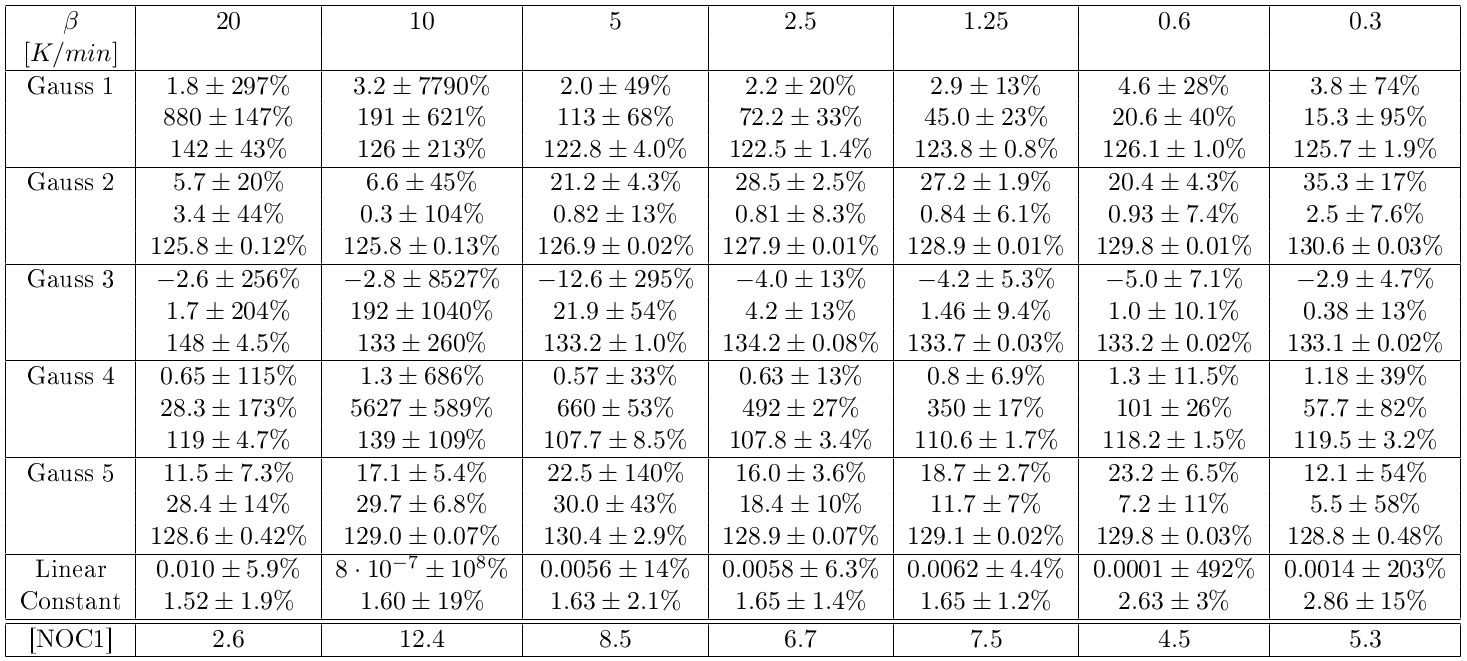
\includegraphics[width=1.\textwidth]{/home/argo/masterarbeit/vortrag/images/stat_a_post_analysis_Gausse.png}
	\end{textblock}	
	
	\begin{textblock}{14}(1.,13.5)
		\begin{itemize}
			\item Probability of error: $5\%$
		\end{itemize}
	\end{textblock}
	
}


\subsection{Fraser-Suzuki parametrization}
\frame{
	\frametitle{Specific heat capacity \& heat flux}	
	\begin{textblock}{14}(1,5)
		\centering
		Heat rate: $10\frac{K}{min}$
	\end{textblock}
	
	\begin{textblock}{14}(1,6.5)
		\includegraphics[width=0.5\textwidth]{/home/argo/masterarbeit/fits_data/2017-12-20_14:25:10_407_L1=40_L3=0,1_N1=300_N3=50_GN_FS_used/2017-12-20_14:30:23_407_10Kmin_L1=40_L3=0,1/c_p_vortrag.png}
	\end{textblock}
	
	\begin{textblock}{14}(8,6.65)
		\includegraphics[width=0.5\textwidth]{/home/argo/masterarbeit/fits_data/2017-12-20_14:25:10_407_L1=40_L3=0,1_N1=300_N3=50_GN_FS_used/2017-12-20_14:30:23_407_10Kmin_L1=40_L3=0,1/heat_flux_vortrag.png}
	\end{textblock}	
	
}


\frame{
	\frametitle{Specific heat capacity \& heat flux}	
	\begin{textblock}{14}(1,5)
		\centering
		Heat rate: $5\frac{K}{min}$
	\end{textblock}
	
	\begin{textblock}{14}(1,6.5)
		\includegraphics[width=0.5\textwidth]{/home/argo/masterarbeit/fits_data/2017-12-20_14:25:10_407_L1=40_L3=0,1_N1=300_N3=50_GN_FS_used/2017-12-20_14:36:33_407_5Kmin_L1=40_L3=0,1/c_p_vortrag.png}
	\end{textblock}
	
	\begin{textblock}{14}(8,6.65)
		\includegraphics[width=0.5\textwidth]{/home/argo/masterarbeit/fits_data/2017-12-20_14:25:10_407_L1=40_L3=0,1_N1=300_N3=50_GN_FS_used/2017-12-20_14:36:33_407_5Kmin_L1=40_L3=0,1/heat_flux_vortrag.png}
	\end{textblock}	
	
}

\frame{
	\frametitle{Statistical a posteriori analysis}	
	
	\begin{textblock}{14}(1.,5.)
		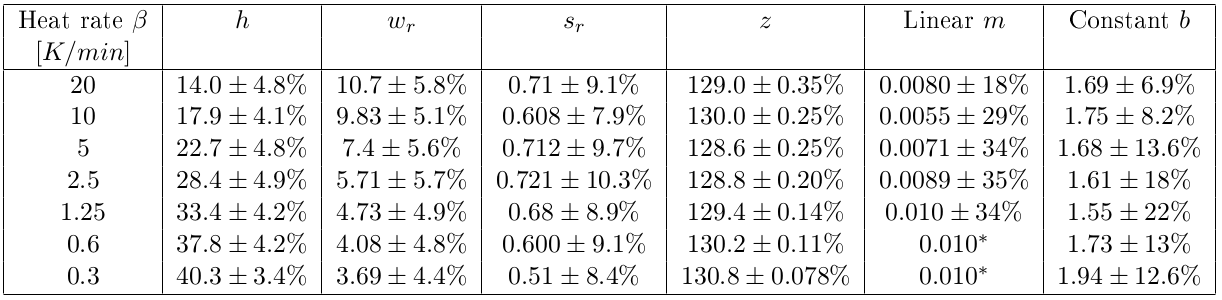
\includegraphics[width=1.\textwidth]{/home/argo/masterarbeit/vortrag/images/stat_a_post_analysis_FS.png}
	\end{textblock}	
	
	\begin{textblock}{15}(0.5,10)
		\begin{itemize}
			\item Probability of error: $5\%$
			\item $^*$ parameter fixed due to lack of measurement data in sensitive part
		\end{itemize}
	\end{textblock}
	
}


\frame{
	\frametitle{Examination of Gauss-Newton iterations}	
	
	\begin{textblock}{8}(0.5,4)
		\includegraphics[width=0.9\textwidth]{/home/argo/masterarbeit/fits_data/2017-12-20_14:25:10_407_L1=40_L3=0,1_N1=300_N3=50_GN_FS_used/2017-12-20_14:36:33_407_5Kmin_L1=40_L3=0,1/optimization_progress.png}
	\end{textblock}
	
	\begin{textblock}{8}(8.5,4)
		\includegraphics[width=0.9\textwidth]{/home/argo/masterarbeit/fits_data/2017-12-20_14:25:10_407_L1=40_L3=0,1_N1=300_N3=50_GN_FS_used/2017-12-20_14:44:53_407_0,6Kmin_L1=40_L3=0,1/optimization_progress.png}
	\end{textblock}
	
}




\subsection{Comparison of retrieved specific heat capacity}

\frame{
	\frametitle{$c_p^{DIN}(T)$ from DIN 11357 formula}
	
	\begin{textblock}{14}(4,5)
		\includegraphics[width=0.6\textwidth]{/home/argo/masterarbeit/vortrag/images/c_p_DIN_formula.png}
	\end{textblock}
	
}


\frame{
	\frametitle{$c_p(T)$ from parameter estimation}	
	
	\begin{textblock}{14}(0.,5.5)
		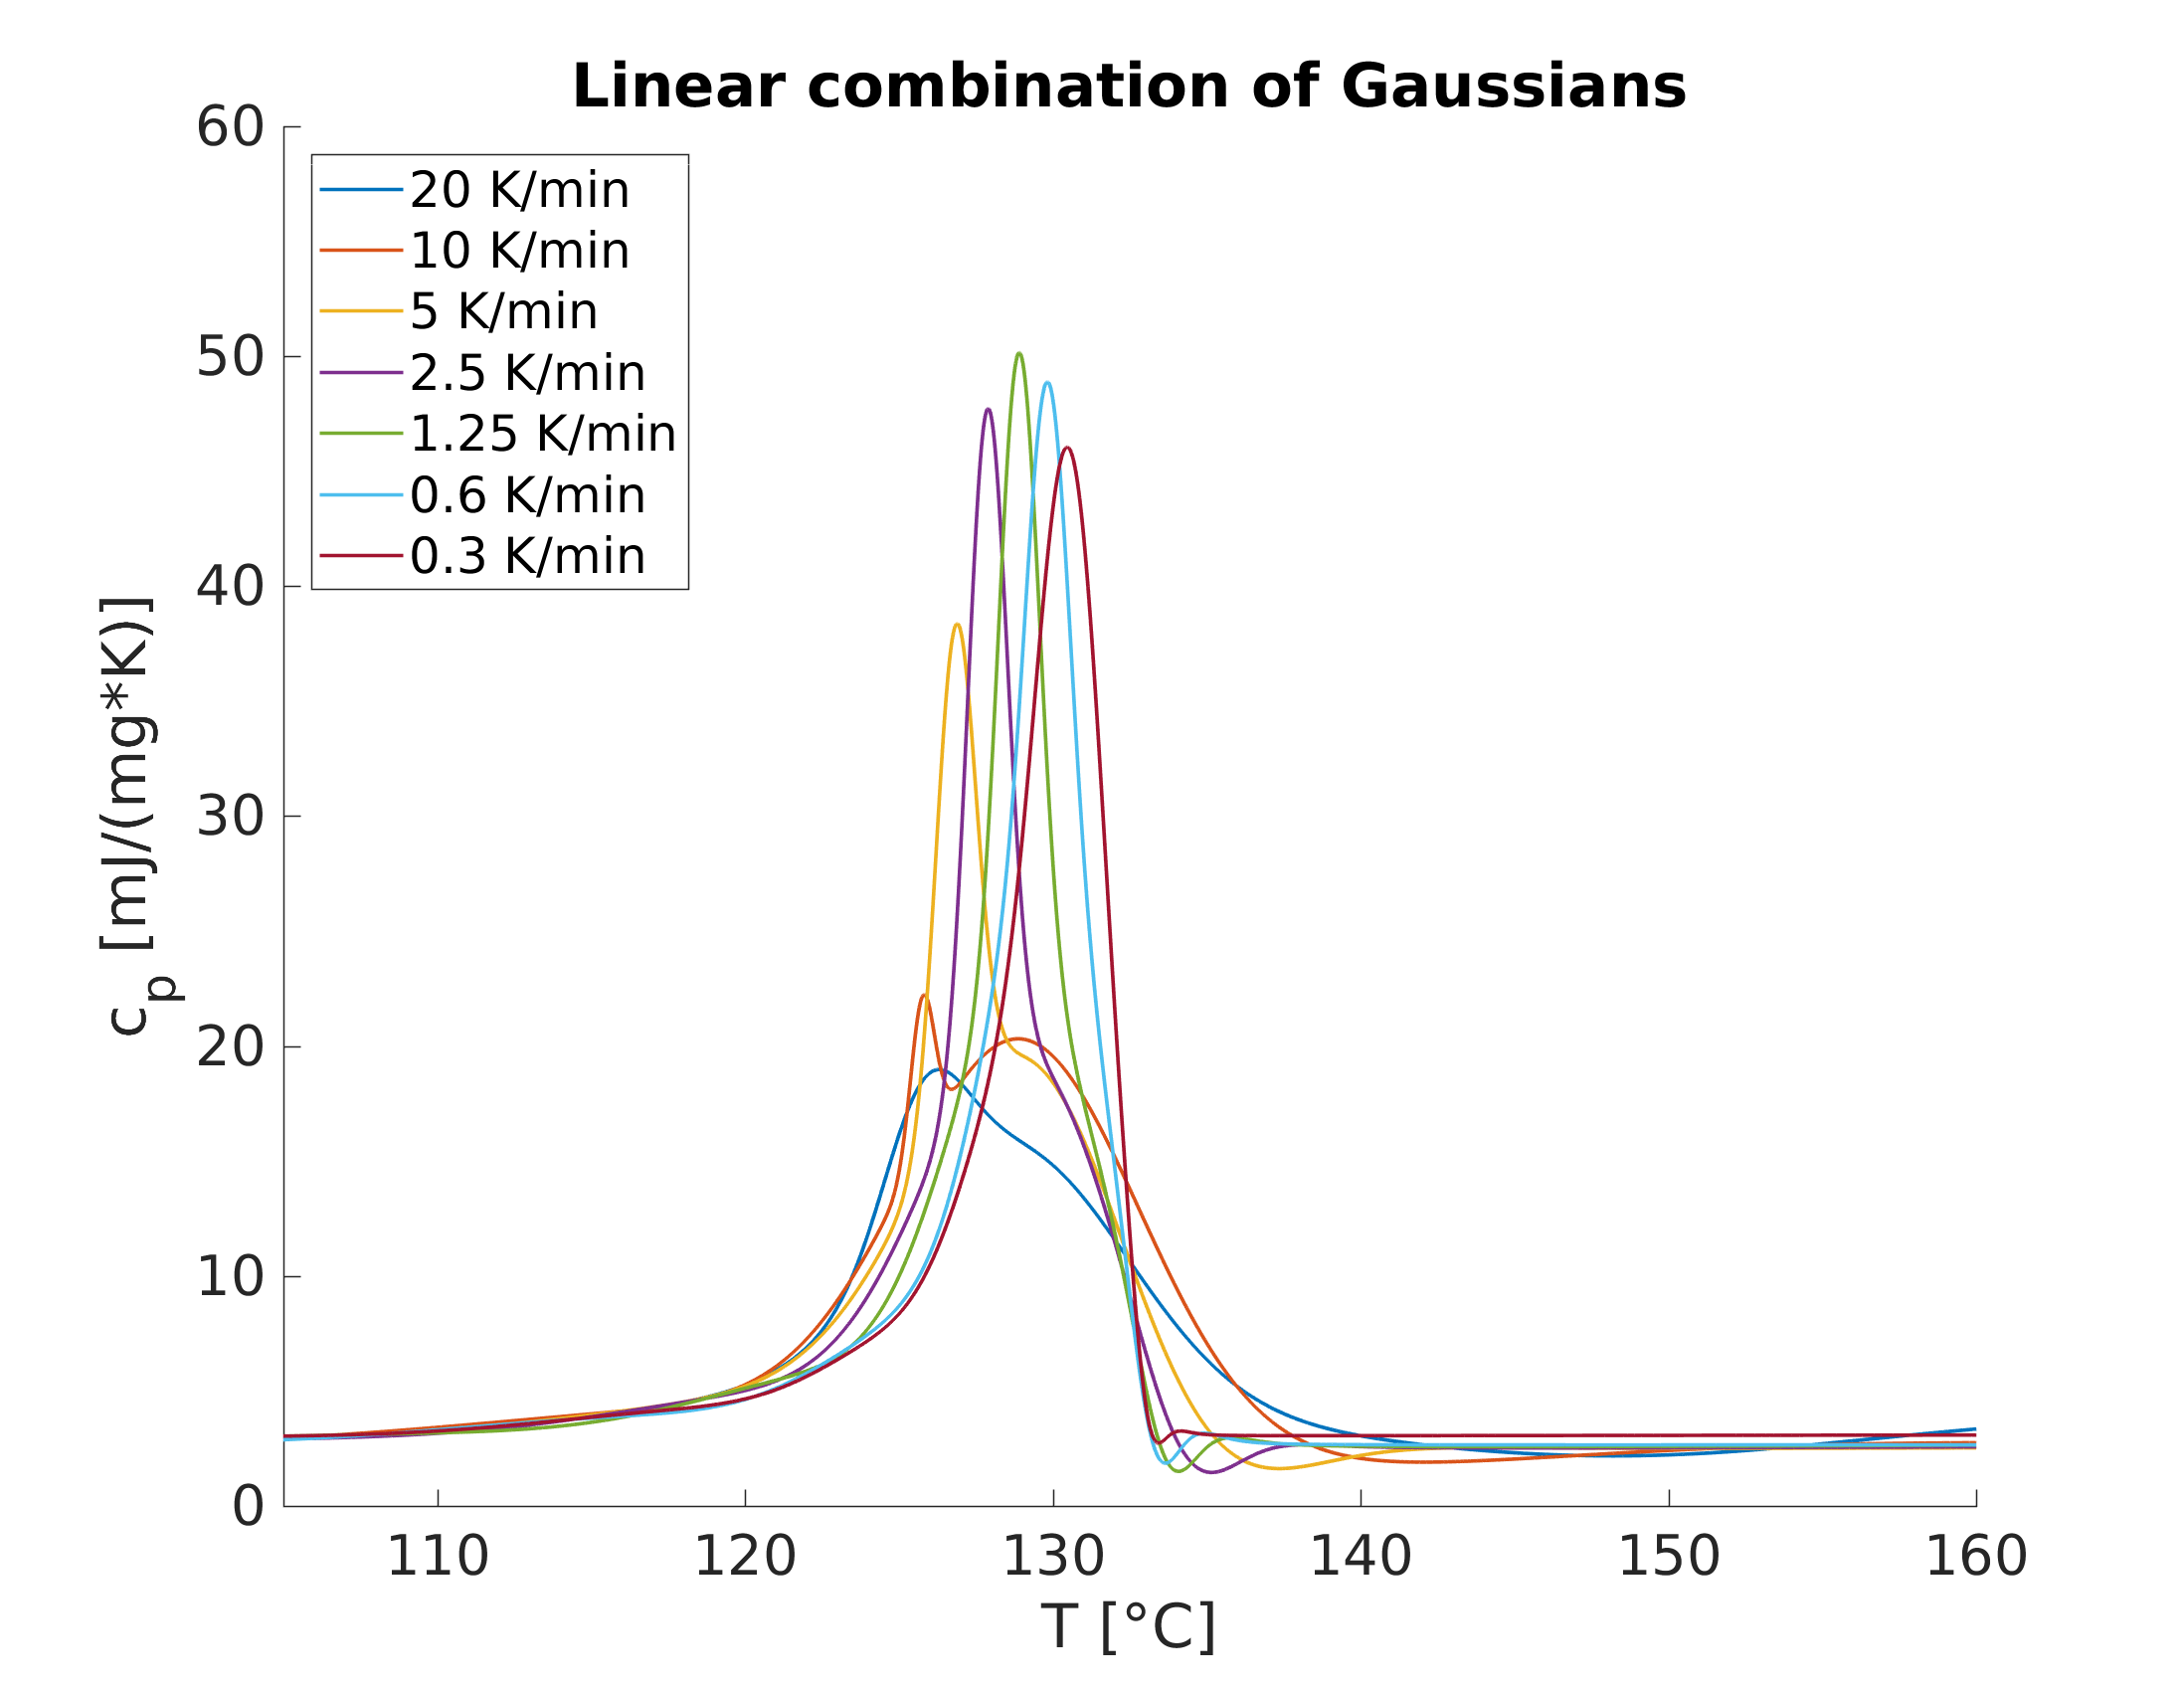
\includegraphics[width=0.6\textwidth]{/home/argo/masterarbeit/vortrag/images/c_p_all_Gaussians.png}
	\end{textblock}
	
	\begin{textblock}{14}(8,5.5)
		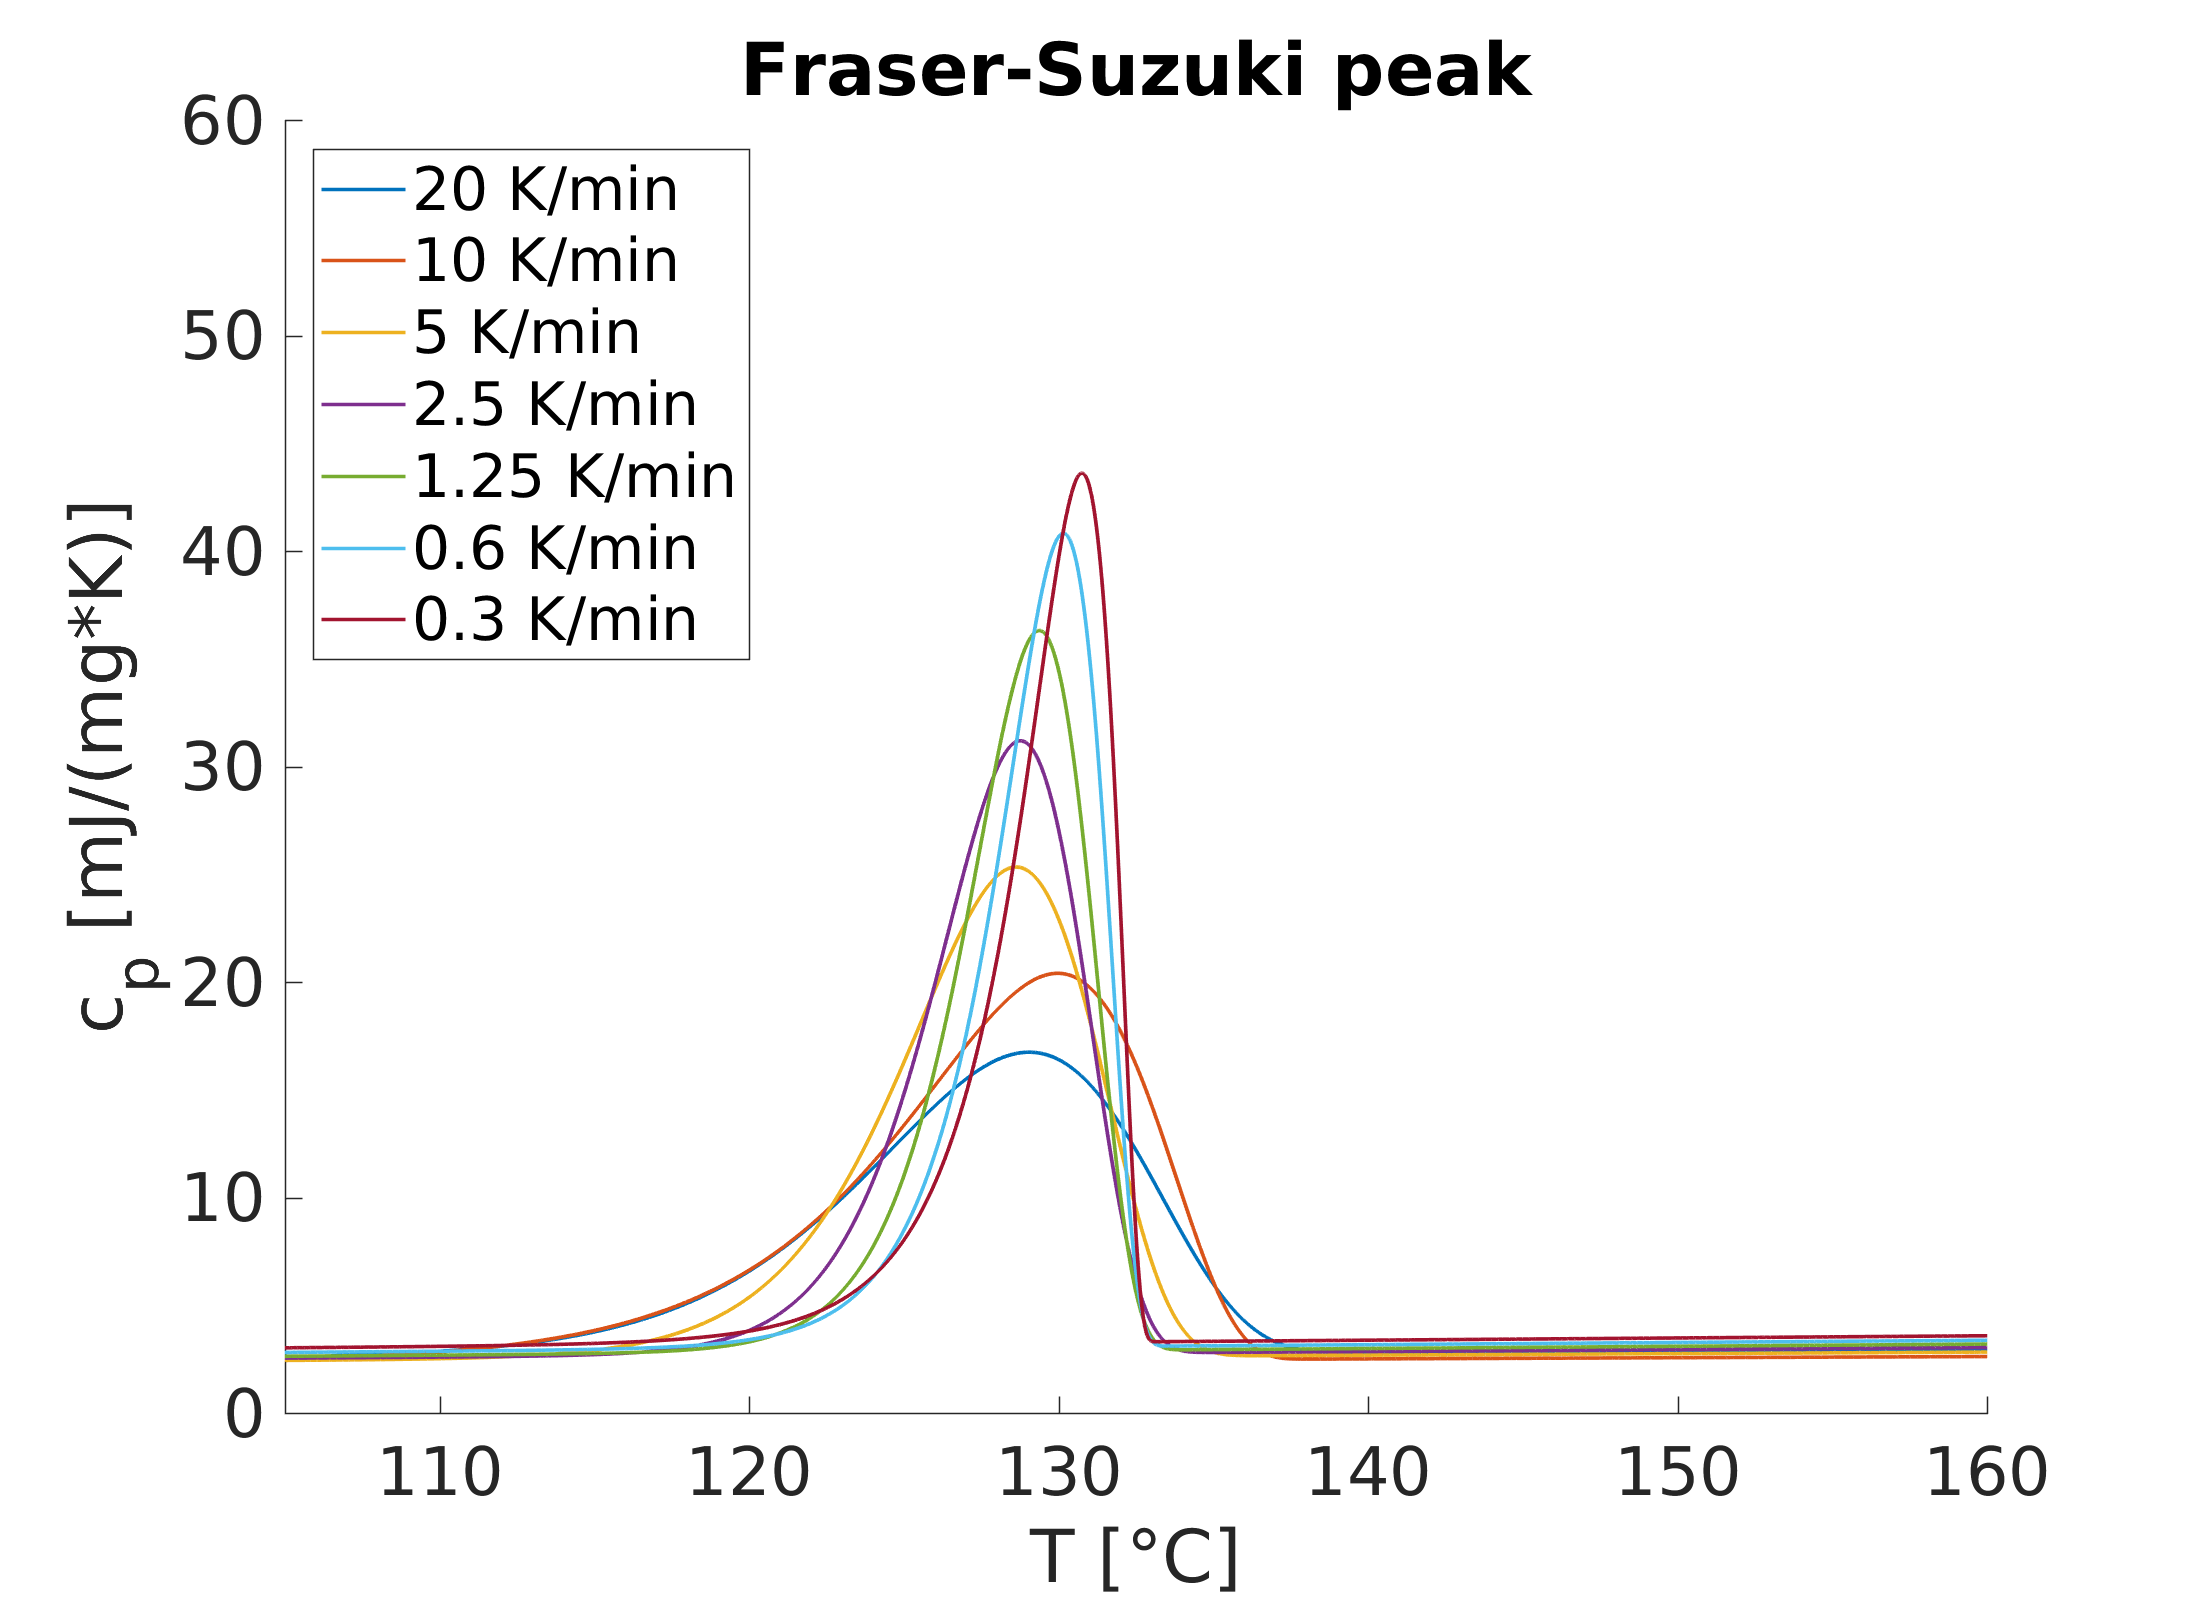
\includegraphics[width=0.6\textwidth]{/home/argo/masterarbeit/vortrag/images/c_p_all_FS.png}
	\end{textblock}
	
}

\frame{
	\frametitle{$c_p(T)$ from parameter estimation}	
	
	\begin{textblock}{14}(0.,5.5)
		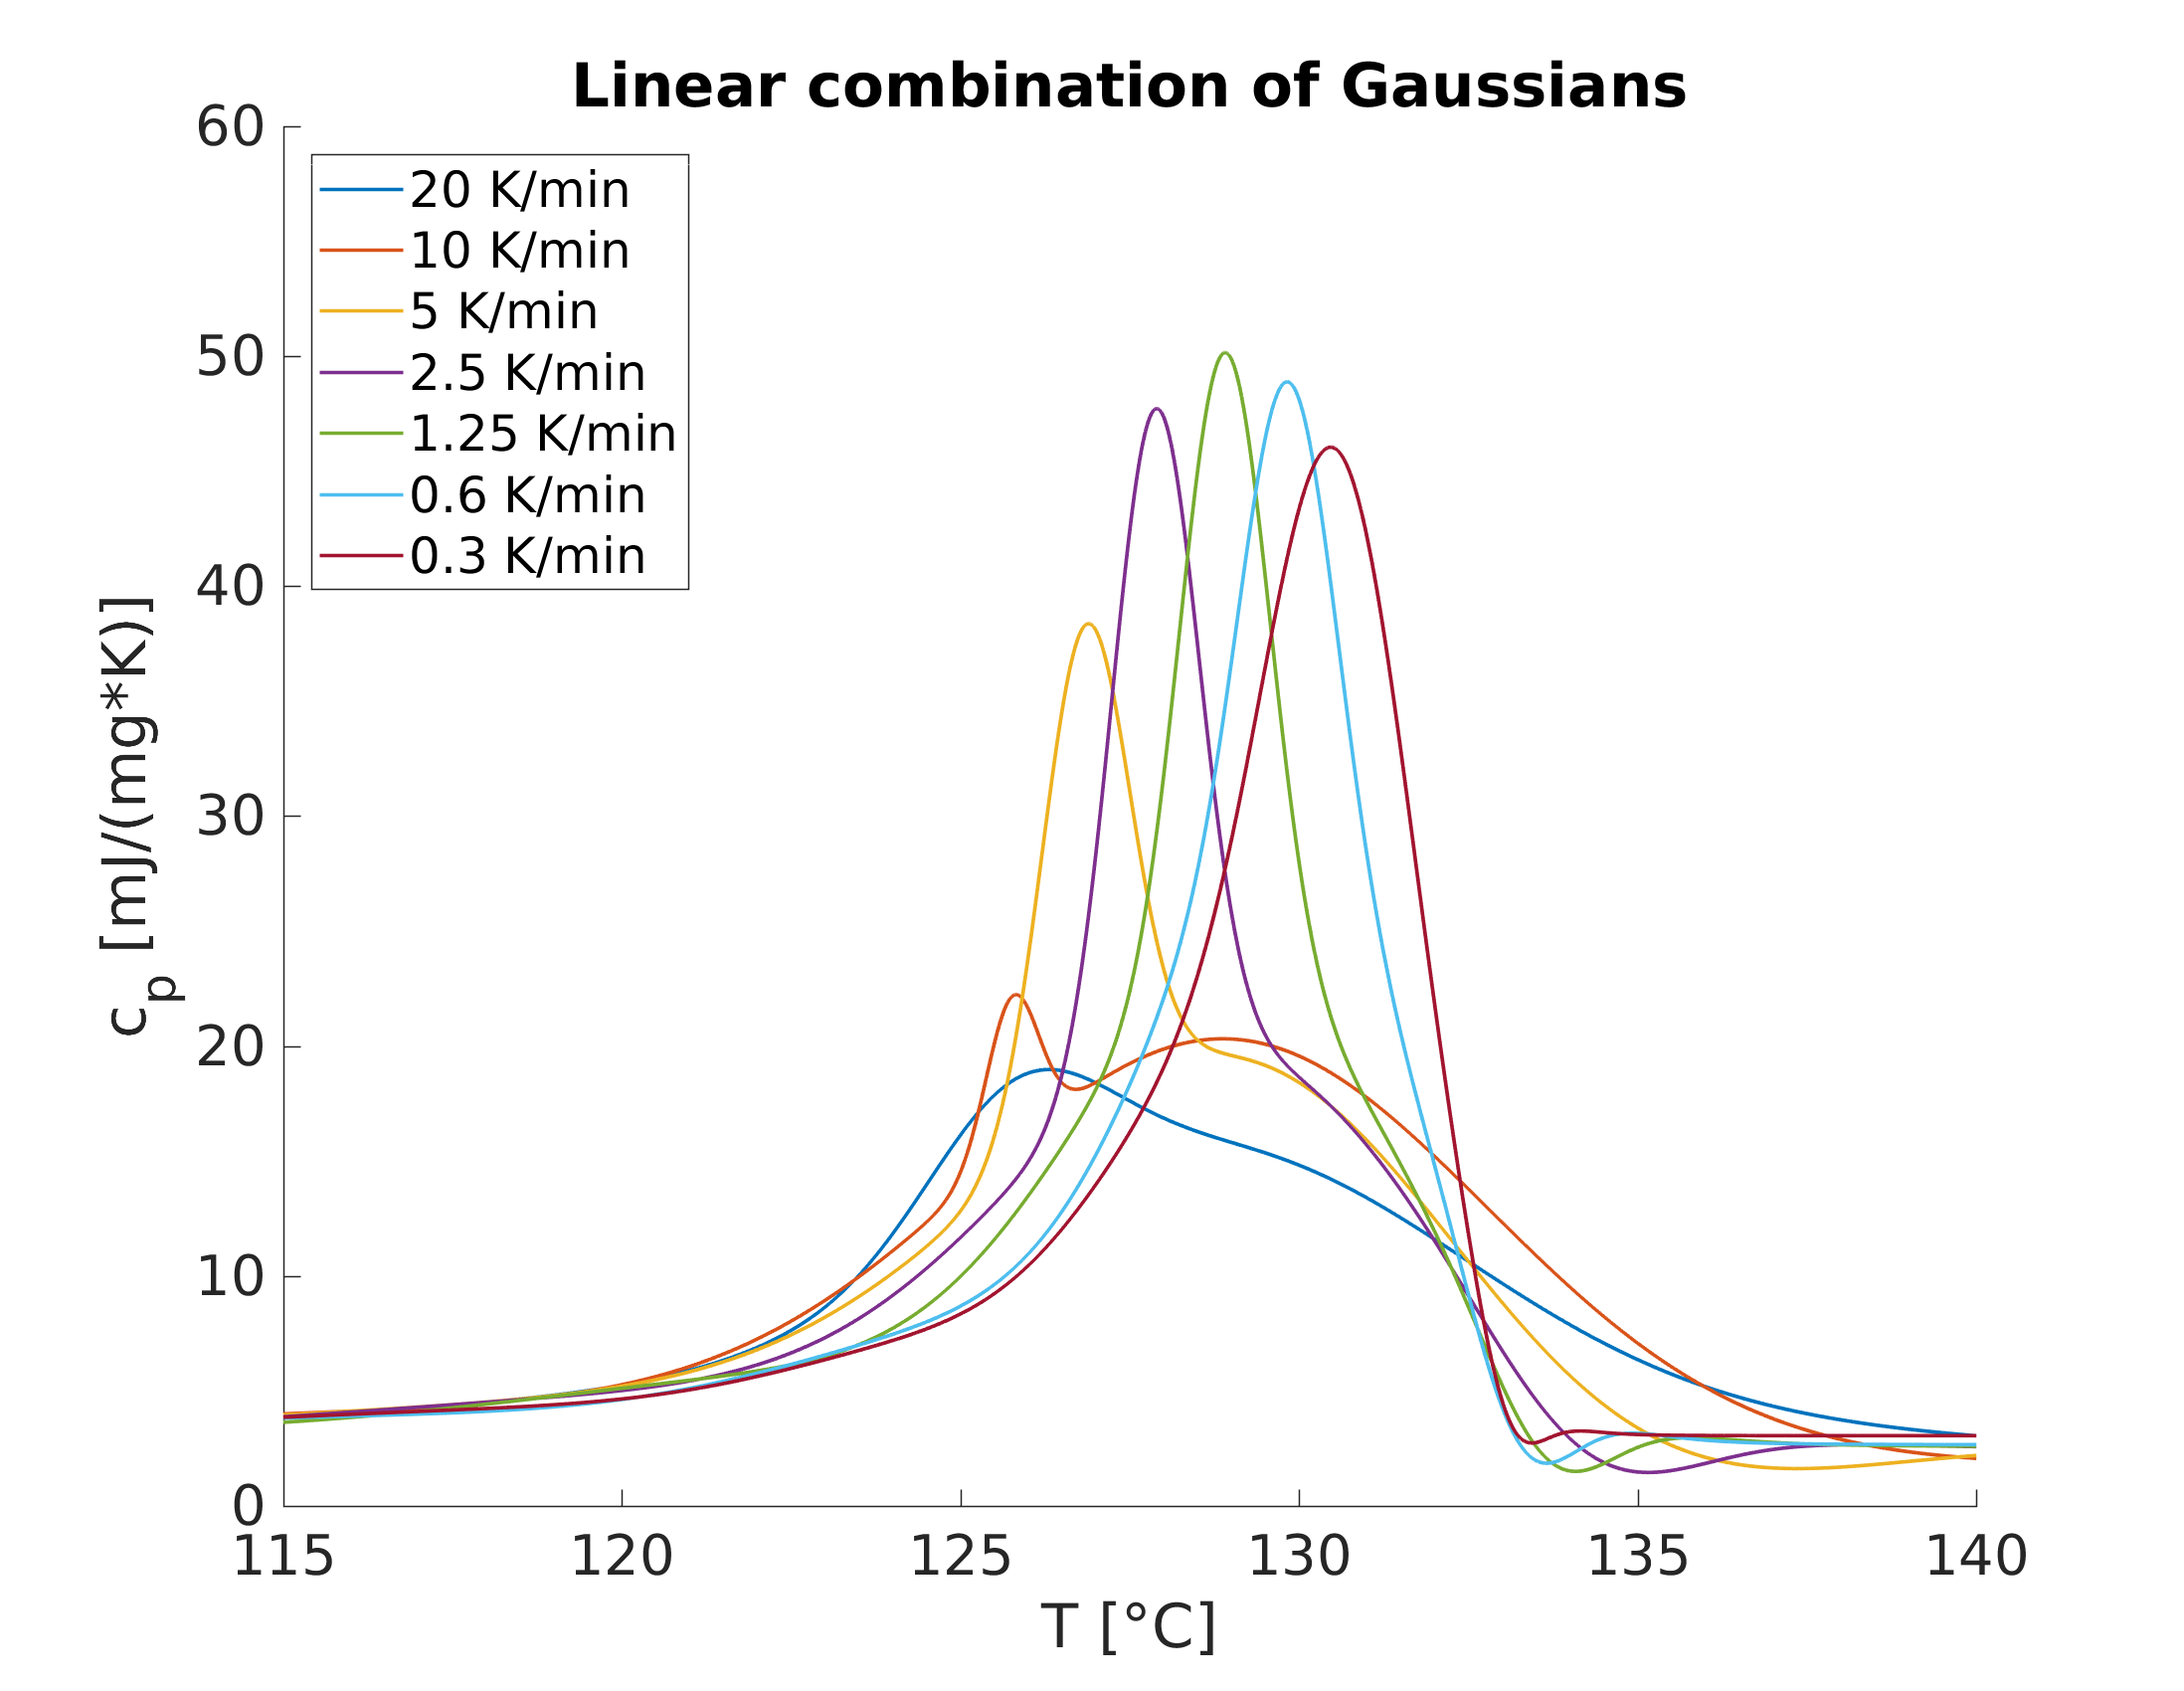
\includegraphics[width=0.6\textwidth]{/home/argo/masterarbeit/vortrag/images/c_p_all_zoom_Gaussians.png}
	\end{textblock}
	
	\begin{textblock}{14}(8,5.5)
		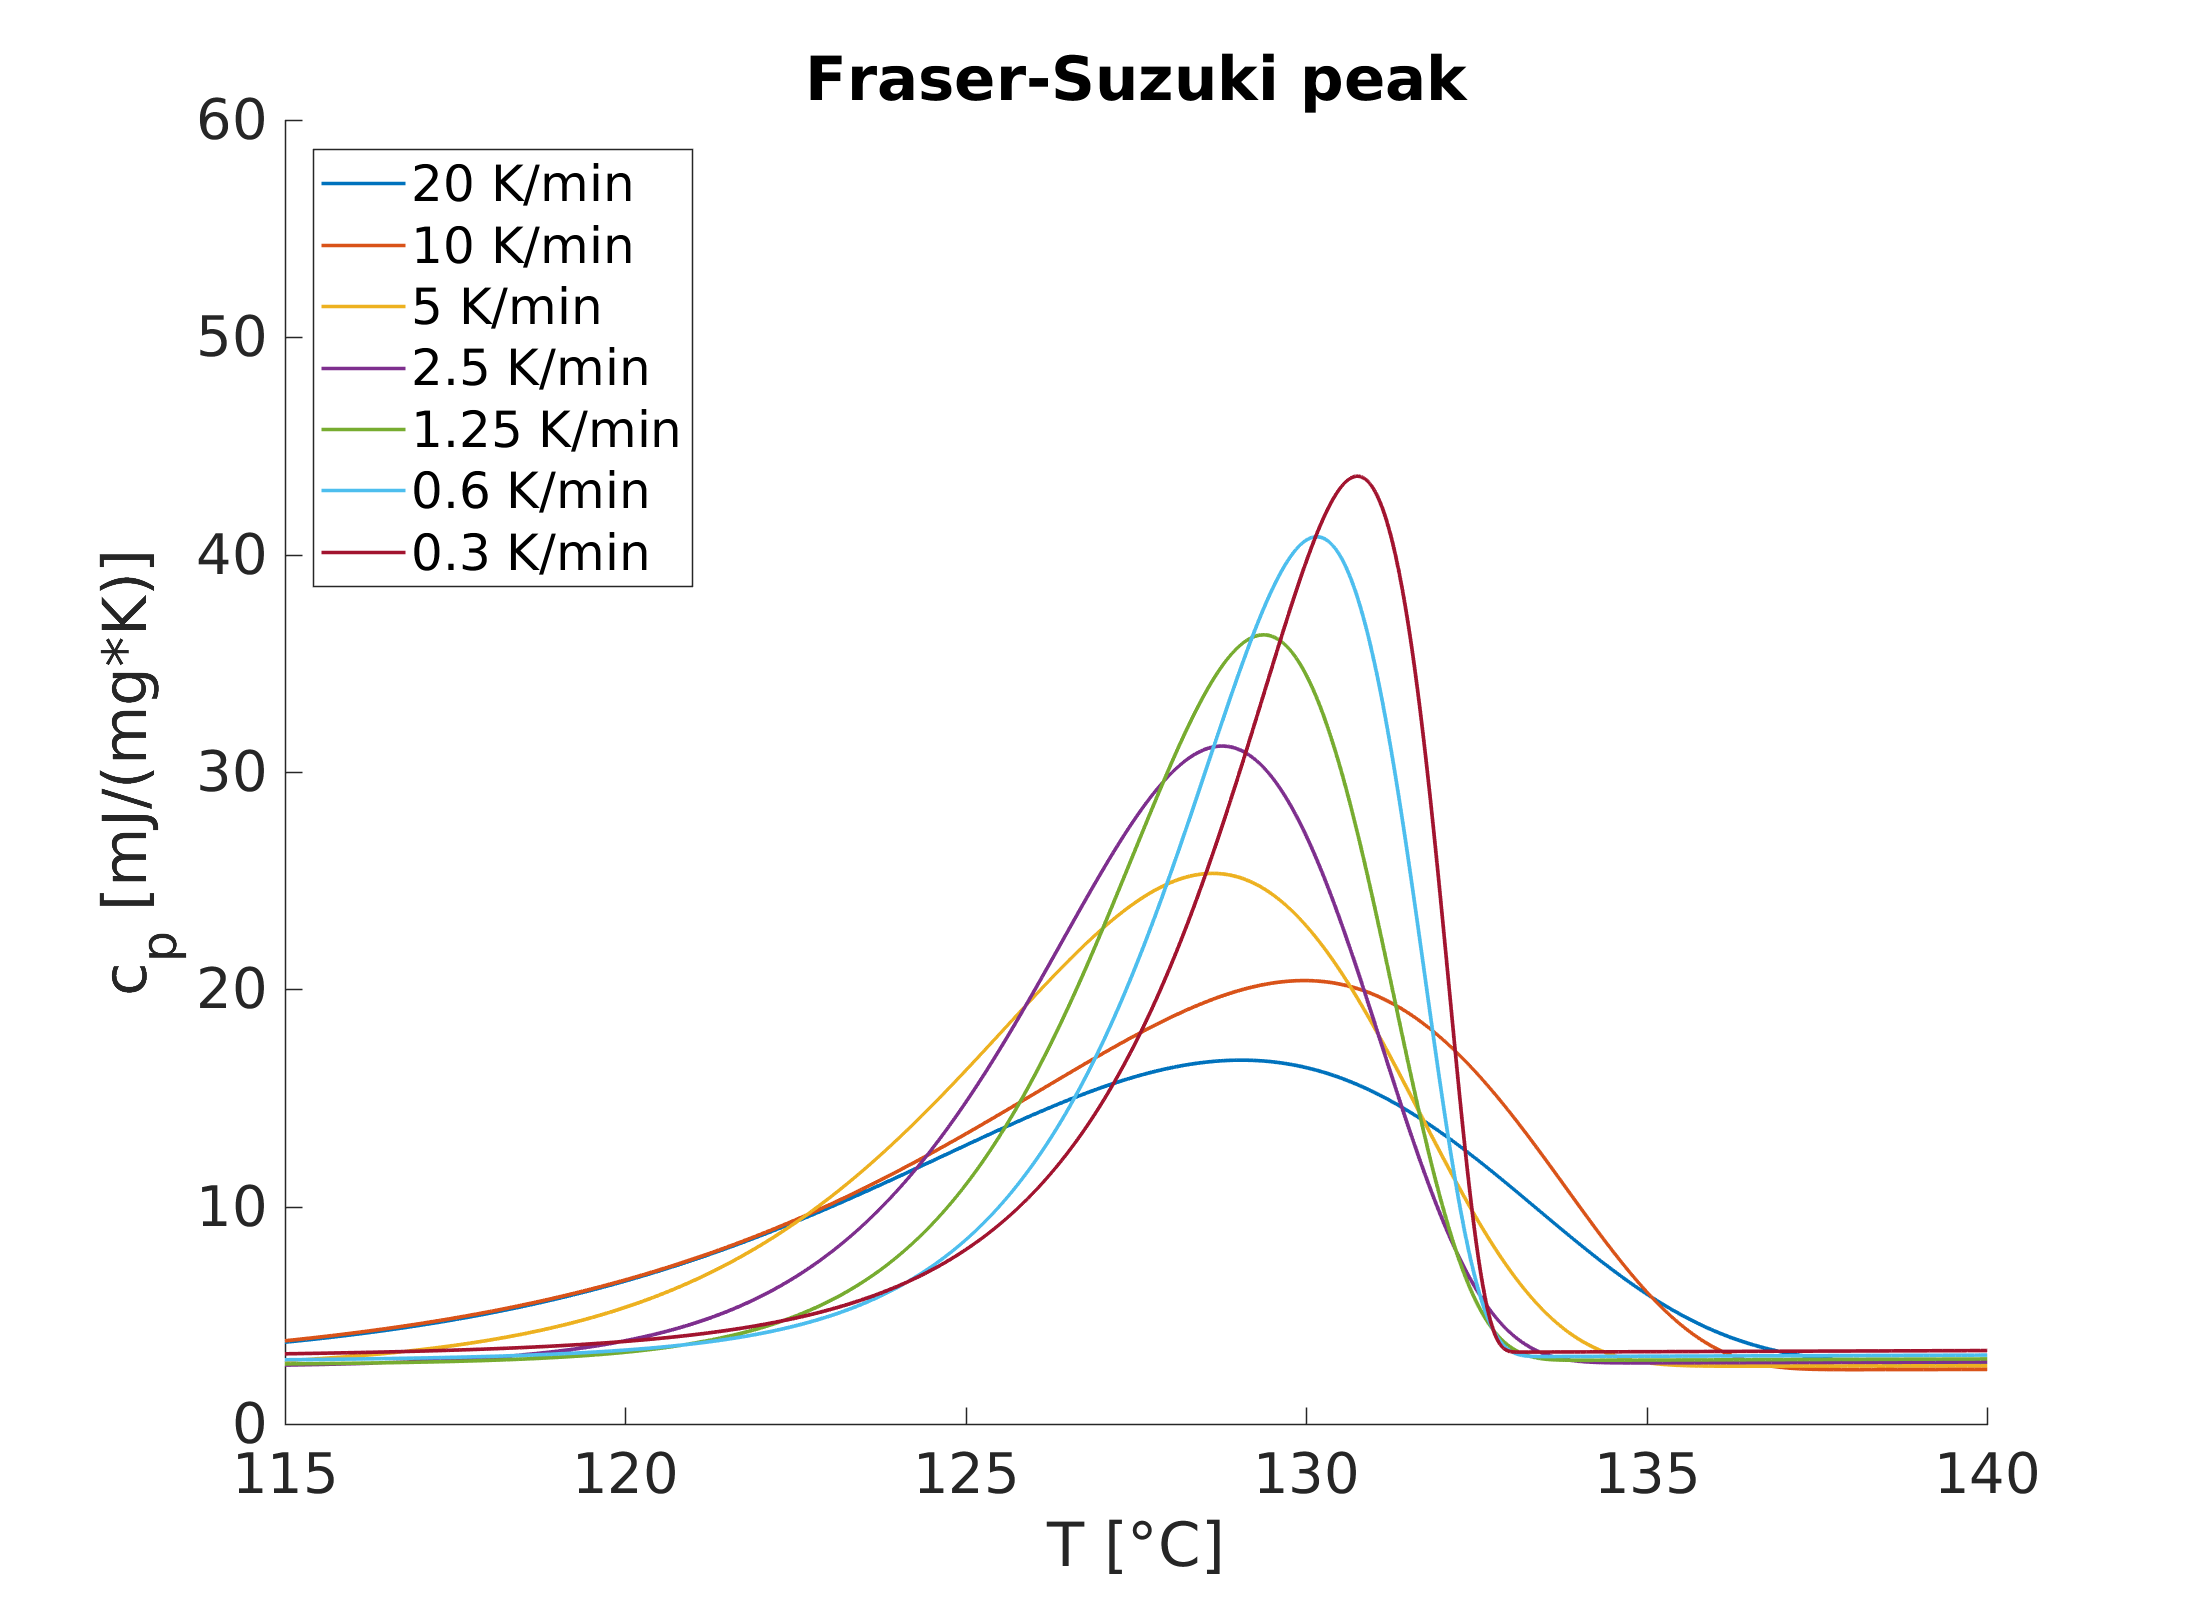
\includegraphics[width=0.6\textwidth]{/home/argo/masterarbeit/vortrag/images/c_p_all_zoom_FS.png}
	\end{textblock}
	
}






\frame{
	\frametitle{Peak characteristics}
	
	\begin{textblock}{13.5}(1.3,4)
		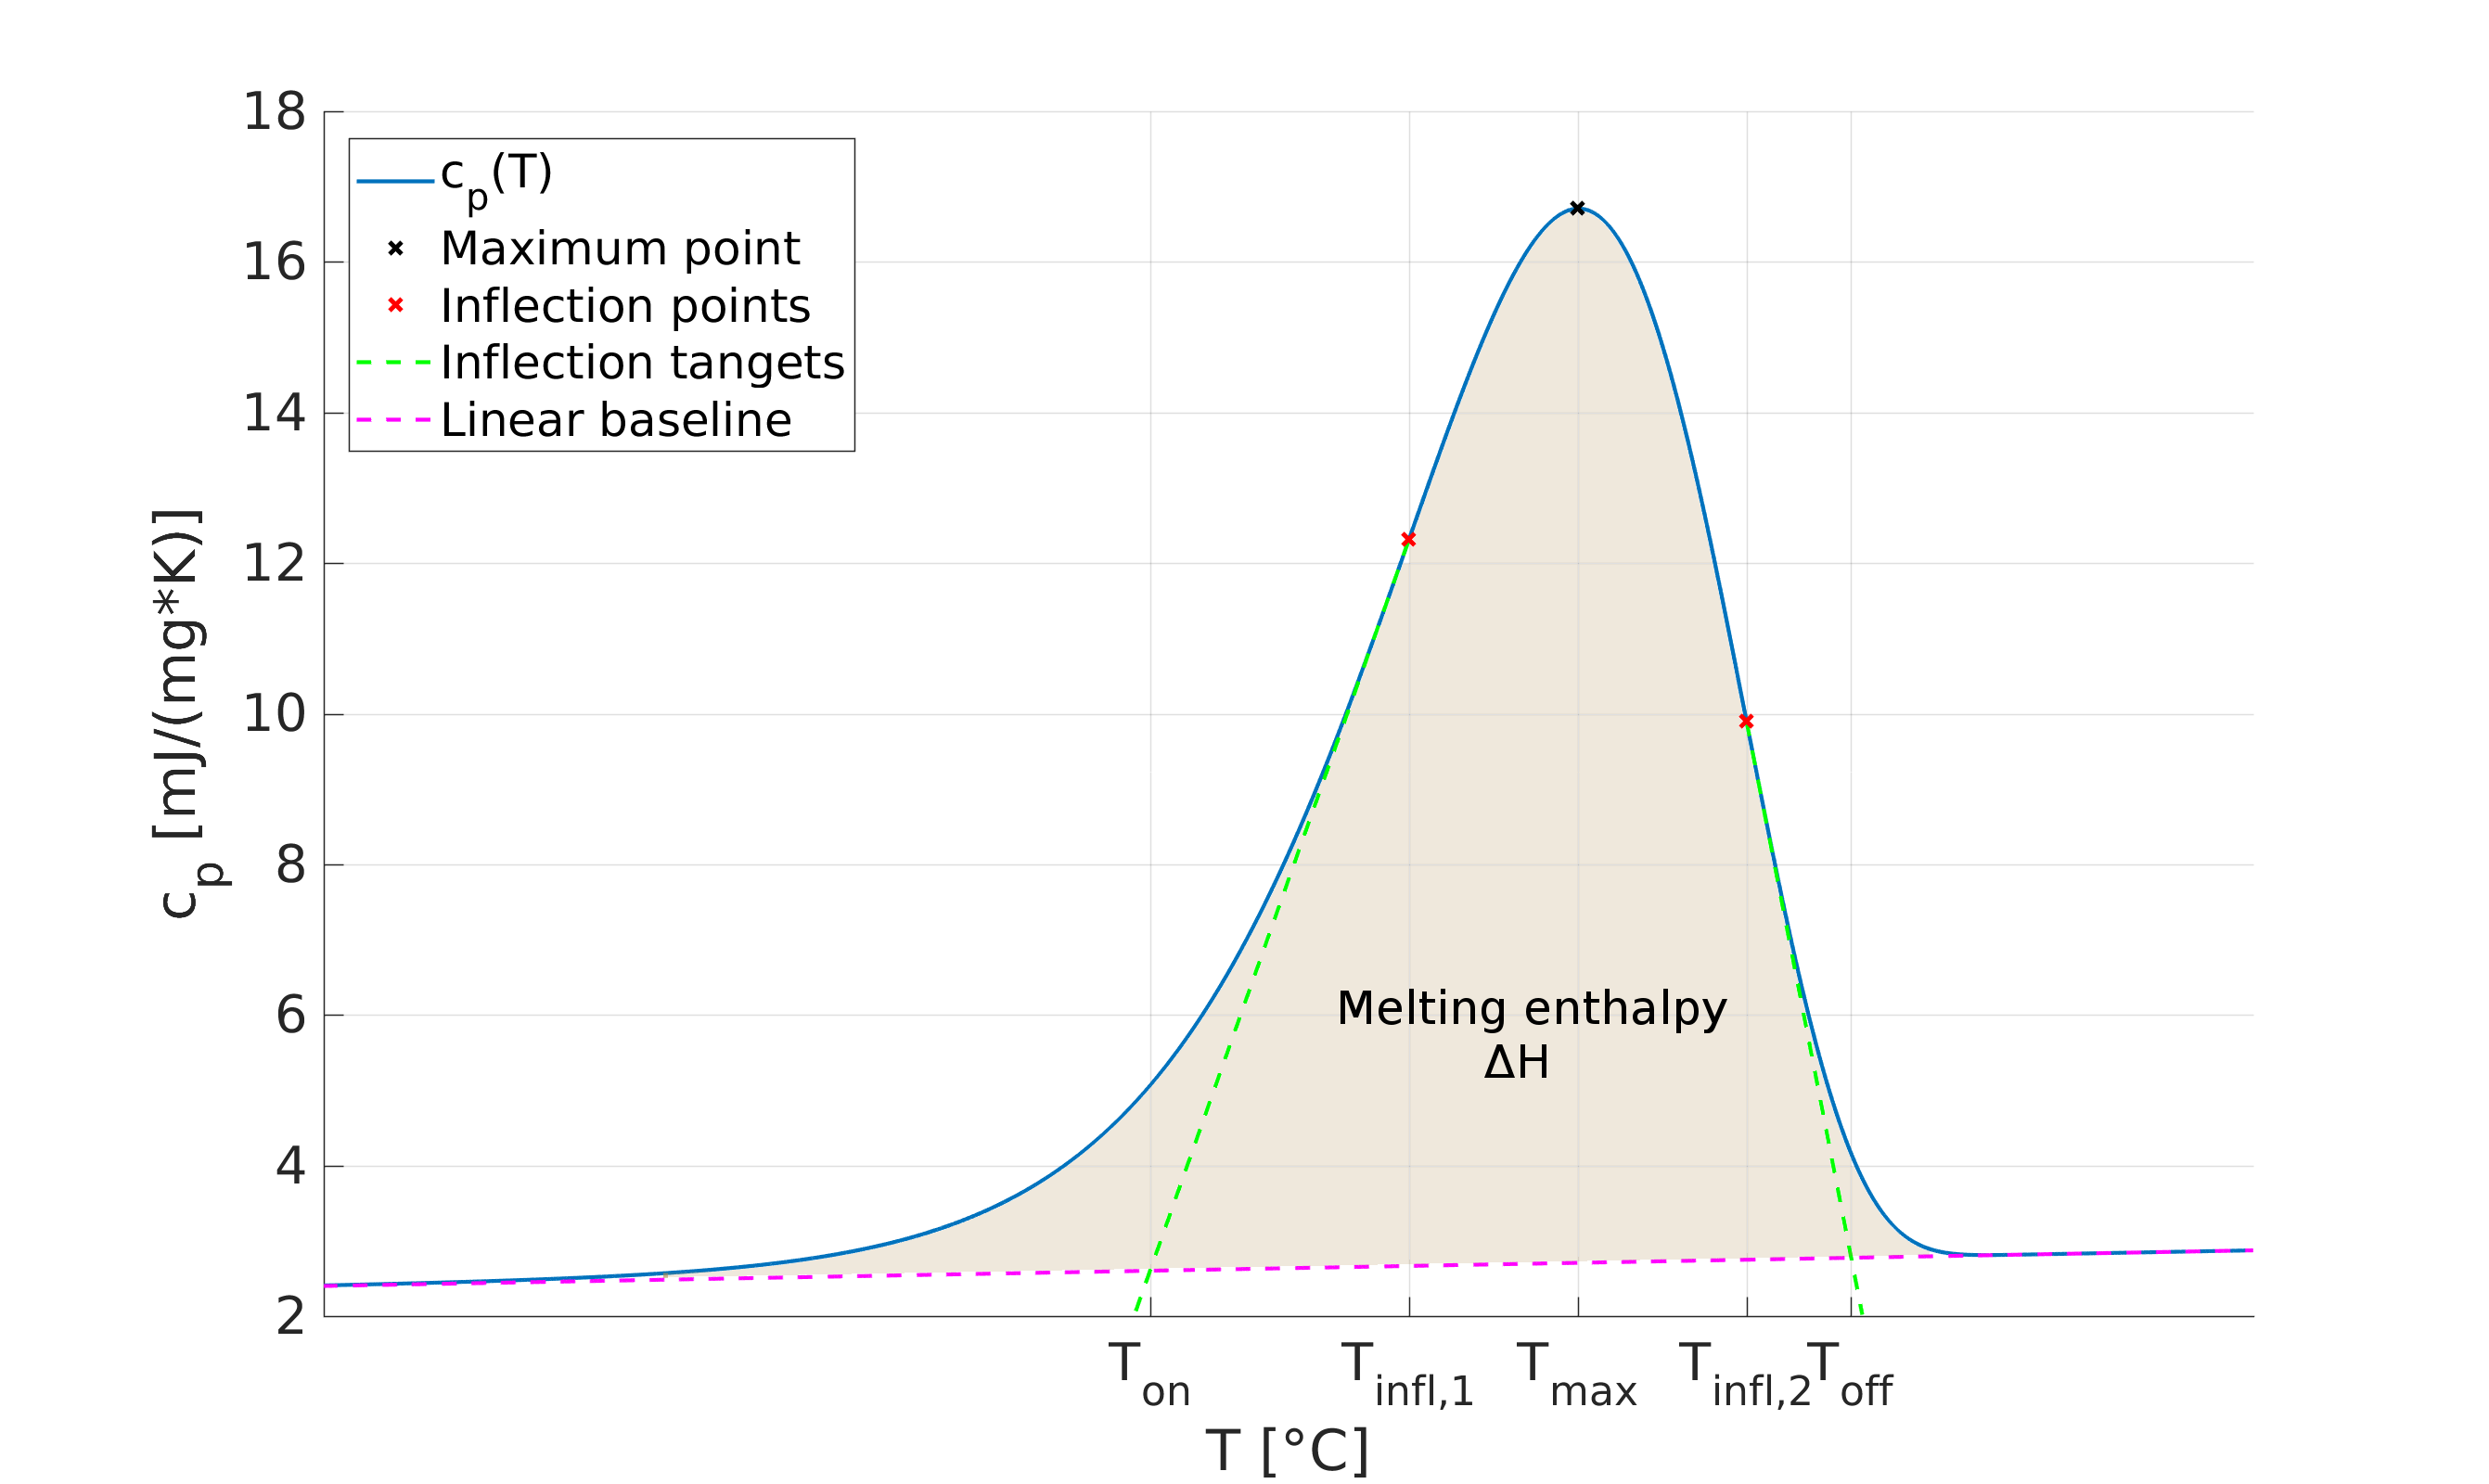
\includegraphics[width=1.\textwidth]{/home/argo/masterarbeit/vortrag/images/T_on_T_off_illustration.png}
	\end{textblock}
	
}


\frame{
	\frametitle{Peak characteristics}
	
	\begin{textblock}{14}(1.,5)
		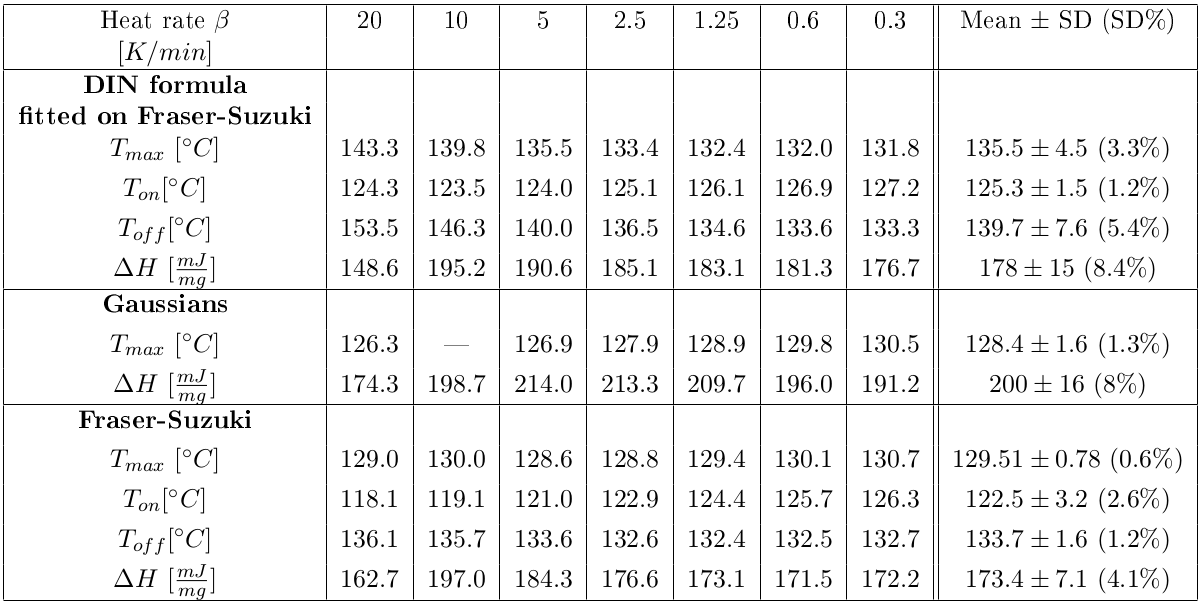
\includegraphics[width=1.\textwidth]{/home/argo/masterarbeit/vortrag/images/summary_peak_characteristics3.png}
	\end{textblock}

}







\section{Possible directions of further research}
\frame{
	\frametitle{Possible directions of further research}
	
	\begin{textblock}{14}(1,4.5)
		\begin{itemize}
			\item Reason for different shape of $c_p$ from optimization?
			\begin{itemize}
				\item Temperature dependent mass density $\rho_{pcm}$? \\
				$\rightarrow$ Mechanical work by volume change has to be considered
				\item Temperature dependent heat conductivity $\lambda_{pcm}$? \\
				$\rightarrow$ Nonlinear term in heat equation
				\item Too simplified model? \\
				$\rightarrow$ 2D model, crucible layer, ...
			\end{itemize}
			\item Reason for NOC1
			\item Reason for integration problems with relative locale error control of forward sensitivities? \\
			$\rightarrow$ Solve variational differential equation
		\end{itemize}
	\end{textblock}	
}

	

\frame{
	
\begin{textblock}{15}(0.5,2.5)
	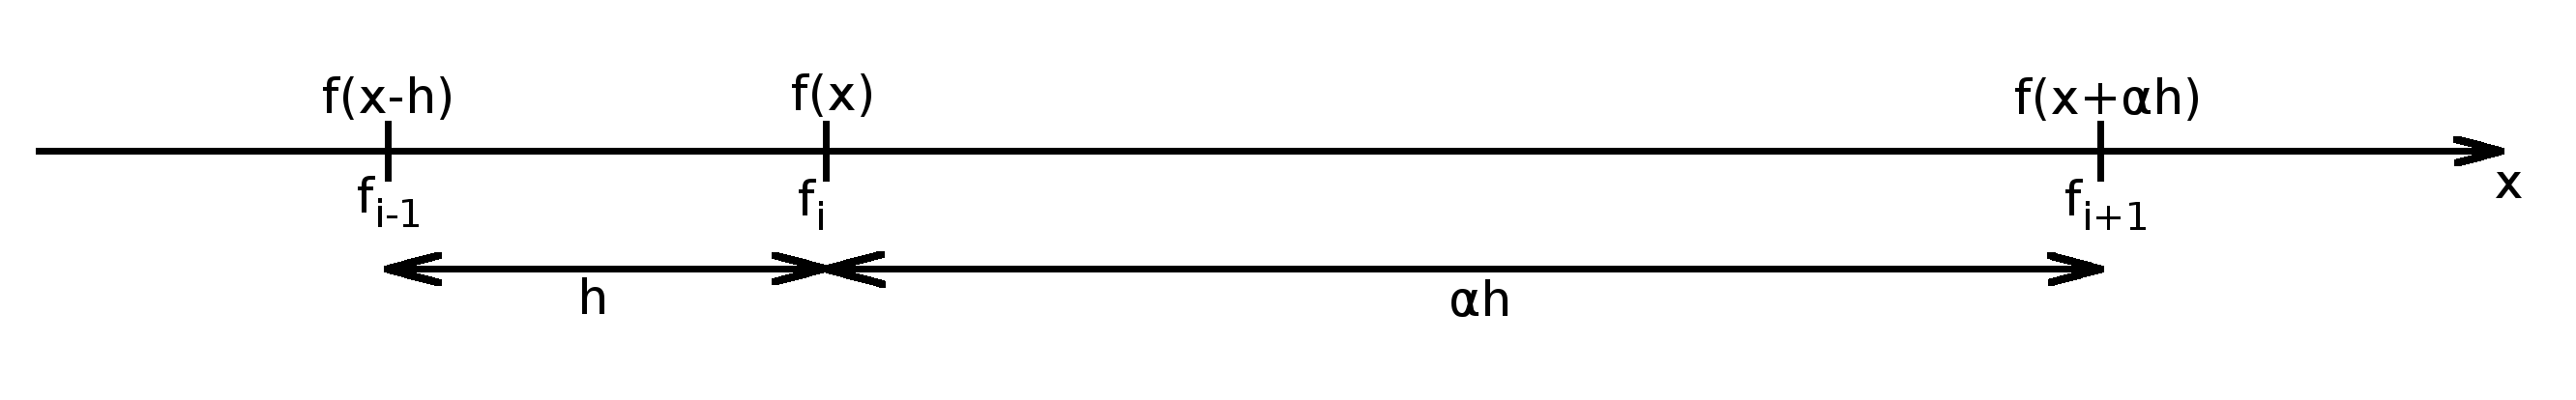
\includegraphics[width=1.0\textwidth]{/home/argo/masterarbeit/thesis/images/2nd_derivative_2-point_formula_illustration.png}
\end{textblock}
	
\begin{textblock}{15}(0.2,6)
	\begin{subequations}
		\begin{align}
		f(x-h) = & f(x) - h \cdot \frac{\partial f}{\partial x}(x) + \frac{h^2}{2} \cdot \frac{\partial^2 f}{\partial^2 x}(x) + \mathcal{O}(h^3) \label{eq:finite_differences_taylor_exp_non-homogenous_1} \\
		f(x+\alpha h) = & f(x) + \alpha h \cdot \frac{\partial f}{\partial x}(x) + \frac{\alpha^2 h^2}{2} \cdot \frac{\partial^2 f}{\partial^2 x}(x) + \mathcal{O}(h^3) \\[3ex]
		\Leftrightarrow \frac{\partial^2 f}{\partial^2 x}(x) = & \frac{1}{h^2} \left[ \frac{2}{1+\alpha} f(x-h) - \frac{2}{\alpha} f(x) + \frac{2}{\alpha (\alpha+1)} f(x+\alpha h) \right] + \mathcal{O}(h^3) 
		\end{align}
	\end{subequations}
\end{textblock}

}
	
\end{document}